\documentclass[thesis=M,czech]{FITthesis}[2012/06/26]

\usepackage[utf8]{inputenc} % LaTeX source encoded as UTF-8

\usepackage{graphicx} %graphics files inclusion
\usepackage{amsmath} %advanced maths
\usepackage{amssymb} %additional math symbols

\usepackage{dirtree} %directory tree visualisation

\usepackage{listings}             % Include the listings-package
\usepackage{color}

\definecolor{dkgreen}{rgb}{0,0.6,0}
\definecolor{gray}{rgb}{0.5,0.5,0.5}
\definecolor{mauve}{rgb}{0.58,0,0.82}

\lstset{frame=tb,
  language=Java,
  aboveskip=3mm,
  belowskip=3mm,
  showstringspaces=false,
  columns=flexible,
  basicstyle={\small\ttfamily},
  numbers=none,
  numberstyle=\tiny\color{gray},
  keywordstyle=\color{blue},
  commentstyle=\color{dkgreen},
  stringstyle=\color{mauve},
  breaklines=true,
  breakatwhitespace=true,
  tabsize=3
}

% % list of acronyms
\usepackage[acronym,nonumberlist,toc,numberedsection=autolabel]{glossaries}
\iflanguage{czech}{\renewcommand*{\acronymname}{Seznam pou{\v z}it{\' y}ch zkratek}}{}
\makeglossaries

\newcommand{\tg}{\mathop{\mathrm{tg}}} %cesky tangens
\newcommand{\cotg}{\mathop{\mathrm{cotg}}} %cesky cotangens

% % % % % % % % % % % % % % % % % % % % % % % % % % % % % % 
% ODTUD DAL VSE ZMENTE
% % % % % % % % % % % % % % % % % % % % % % % % % % % % % % 

\department{Katedra softwarového inženýrství}
\title{Umístění dat na výpočetní uzly minimalizující datové přenosy v databázi HBase}
\authorGN{Miroslav} %(křestní) jméno (jména) autora
\authorFN{Hrstka} %příjmení autora
\authorWithDegrees{Bc. Miroslav Hrstka} %jméno autora včetně současných akademických titulů
\supervisor{Ing. Adam Šenk}
\acknowledgements{Děkuji Ing. Adamovi Šenkovi za vedení diplomové práce, cenné připomínky a rady, které příspěly k úspěšnému vypracování této práce. Poděkování patří také Pavle Přibylové za nemalou pomoc s formální stránkou práce. }
\abstractCS{	Tato práce si dává za cíl zmapovat možnosti optimalizace datových přenosů v databázi HBase. Je analyzováno stávající řešení navržené pro souborový systém HDFS. Na základě zjištěných skutečností je zvážena možnost použít principiálně podobné schéma optimalizace pro HBase a následně je toto řešení navrhnuto a naimplementováno. Výsledek optimalizace je nutné následně otestovat a vyhodnotit.}
\abstractEN{This work is aimed to map out the options for optimizing data transfers in the database HBase. It analyzed existing solutions designed for HDFS file system. Based on these findings is considered to use principally similar pattern and apply it to the HBase database.  Subsequently, this solution is designed and is deployed. At the end the result of optimization is need to be tested and evaluated.}
\placeForDeclarationOfAuthenticity{V~Praze}
\declarationOfAuthenticityOption{4} %volba Prohlášení (číslo 1-6)
\keywordsCS{HBase, Hadoop, distribuované databáze, optimalizace}
\keywordsEN{Hbase, Hadoop, distributed database, optimization}

\begin{document}
\lstset{language=sh}  
% \newacronym{CVUT}{{\v C}VUT}{{\v C}esk{\' e} vysok{\' e} u{\v c}en{\' i} technick{\' e} v Praze}
% \newacronym{FIT}{FIT}{Fakulta informa{\v c}n{\' i}ch technologi{\' i}}

\begin{introduction}
Pojem databáze se pojí s informačními technologiemi prakticky od vzniku tohoto oboru. Samotná touha a potřeba ukládat data v nějaké strukturované podobě zde byla tisíce let před vynalezením počítače a nasazení počítačů bylo jen logickým pokračováním vývoje správy dat. Dlouhou dobu se uložení dat řešilo pomocí relačních databází, kde princip uložení dat zůstával víceméně stejný, jen docházelo ke zvyšování výkonu a zvětšování kapacity uložišť.

 V posledních letech však stoupá tlak na maximální využití všech dostupných datových zdrojů, jejichž množství stále roste. To vede k potřebě skladování obrovského množství dat. Tato data nicméně nebývají vždy strukturovaná a mohou být i semistrukturovaná nebo nestrukturovaná. Mezi tyto data lze zahrnout různé logy, textové soubory nebo i částečně strukturovaná data, která nemají zcela pevnou strukturu. Zároveň je zde ale i požadavek na co nejnižší náklady na systémy sloužící k uložení těchto dat. Pro tento typ dat a pro takové množství už přestaly být relační databáze vhodným řešením a právě tato poptávka dala za příčinu rozvoji takzvaných NoSQL databází. NoSQL je pojem, který zastřešuje databáze, které pracující na jiném principu než relační databáze, především sloupcově orientované databáze, key/value databáze a další. 
 
 
Mezi nejvýznamější reprezentanty této skupiny patří právě platforma Hadoop a databáze HBase. Hadoop je distribuovaná platforma určená pro zpracování dat v řádech petabytu až exabytů a pro zpracování takového množství dat využívá v praxi desítky až stovky výpočetních uzlů. Proto je navržena právě tak, aby mohl být pro realizaci použitý běžný komoditní hardware a bylo tak možné pořídit uložiště co nejlevněji. Z tohoto řešení vyplývají i jistá omezení. Ta se projevují především v rychlosti zpracování. To ale pro zpracování analytických dat, pro které tyto databáze typicky slouží, není klíčovým měřítkem.


Hadoop a zároveň i databáze HBase stojí na zpracování dat pomocí frameworku MapReduce, ten se řídí principem přenosu instrukcí za daty a tím se výrazně minimalizuje přenos dat mezi uzly výpočteního clusteru. MapReduce není nová myšlenka, ale teprve Hadoop umožnil používat tento systém v širší praxi a na větším spektru úloh.


Ikdyž se Hadoop a HBase vyznačují nízkými přenosy dat během provádění dotazů, zejména díky lokalizaci dat, je zde stále prostor pro zlepšení. Taková úspora přenosové kapacity mezi clustery by mohla nastat při optimálním rozložení dat na discích tak, aby byla co nejideálněji seskupena data, která jsou společně zpracovávána stejným redukčním uzlem v rámci MapReduce. A právě najít a provést takovéto rozdělení pro data uložená v databázi HBase je cíl stanovený pro tuto práci, protože i malá procentuální úspora přenosů dat mezi výpočetními uzly v kombinaci s nižší propustností používaných běžných síťových prvků, vyššími přístupovými dobami pevných disků a velkými objemy zpracovávaných dat může výrazně snížit časovou náročnost často vykonávaných dotazů. 


\end{introduction}
\chapter{Data a Databáze}
Na začátku, dříve než budou představeny detailní nástroje se kterými se bude pracovat, je na místě provést stručné vysvětlení základních pojmů a uvést trochu teorie. 
\section{Data}
Jedná se o pojem prolínající se celou prací. Pod tímto pojmem se schovává poměrně abstraktní veličina. Jako nejvhodnější definice v kontextu této práce se mi jeví následující popis:

\medskip
\textit{"Pojem data vychází z latinského slova datum, které lze vyložit jako něco daného a které
bylo původně odvozeno z příčestí minulého slova dare, tedy dát. V kontextu počítačové
vědy se pojem data vždy používal jako označení pro čísla, text, zvuk, obraz, popř. jiné
smyslové vjemy reprezentované v podobě vhodné pro zpracování počítačem."} \cite{data}
\medskip

Dále se tedy zde bude nahlížet na data pouze v rámci informačních technologií. To, co je z pohledu nahlížení na data v této práci důležité, je jejich vlastnost, jak jsou zpracovatelná. Podle zpracovatelnosti lze data rozdělit do třech skupin:
\begin{itemize}
\item \textbf{Strukturovaná data} jsou uspořádáná podle pevně daného formátu. Typicky se jedná o data uložená v tabulkách.

\item \textbf{Nestrukturovaná data} naopak nemají žádný pevný formát. Příkladem nestrukturovaných dat mohou být knihy, dokumenty, audio, video, obrázky nebo analogová data.

\item \textbf{Semistrukturovaná data} sice nepodléhají pevně danému schématu, i přesto se u nich v určité podobě projevuje uspořádání, nebo ne striktně pravidelná struktura, která se může měnit nepredikovatelným způsobem. Jedná se například o XML nebo JSON soubory nebo logy z webových serverů.
\end{itemize}
 

\section{Databáze}
Obecně se pod slovem databáze myslí uspořádaná množina dat, uložená na nějakém paměťovém médiu. V širším smyslu se jako databáze označují i softwarové prostředky, které s těmito daty umožňují manipulovat. Tento celek se pak nazývá DBMS (Database management systems). Existuje mnoho druhů databází, v zásadě je ale můžeme rozdělit na dvě hlavní skupiny:

\begin{itemize}
\item SQL Databáze
\item NoSQL Databáze
\end{itemize}

Dlouhou dobu zaujímaly výsadní postavení na trhu relační databáze spadající do SQL databází. Nicméně právě nové trendy dávají poslední dobou prostor k většímu využívání NoSQL databází.

\subsection{SQL Databáze}
Ačkoli se v práci nebude pracovat s SQL databázemi, nelze je nezmínit hlavně z důvodu porovnání oproti NoSQL databázím. Jen ve stručnosti budou uvedeny hlavní rysy většiny SQL databází. SQL databázemi jsou označovány databáze, které umí zpracovat dotazy v jazyku SQL. Jedná se především o relační databáze a tak i tato kapitola bude zaměřená právě na ně.

Relační databáze ukládají data do tabulek, které mají mezi sebou pevně definované vztahy. Tabulky mají pevný počet předem daných sloupců a data se ukládají po řádcích. Sloupce mají jedinečný identifikátor a určený datový typ. Každá buňka tabulky může obsahovat jen jednu hodnotu. V případě, že je zapotřebí do jedné buňky vložit více hodnot, je nutné tabulky propojit pomocí primárních a cizích klíčů. Díky omezené variabilitě ukládaných dat a nutnosti dodržovat striktní formát tabulek je umožněno pomocí jazyku SQL vytvářet nad tabulkami komplexní dotazy.


\subsection{NoSQL Databáze}
Původně se tímto názvem označovaly databáze, které jak již z názvu vyplývá, nevyužívají pro práci s daty SQL jazyk. Nyní se volí jako správný výklad NoSQL "Not Only SQL" a do této množiny zapadají všechny databáze, které nejsou postaveny na relačním principu.  NoSQL databáze se vyznačují menší komplexicitou při vytváření dotazů, často se omezující pouze na vkládání, čtení a mazání záznamů. Tato komplexicita je však kompenzována vysokou optimalizací pro vyhledávání. Oproti relačním databázím jsou o mnoho škálovatelnější a tak se může lépe využít pro ukládání velkého množství dat, která neustále přibývají. Škálovatelnost NoSQL databází vyplývá především z faktu, že není potřeba zachovávat vzájemné vztahy mezi tabulkami.

NoSQL databáze mají typicky distribuovanou architekturu, která v kombinaci s replikacemi dat poskytuje dostatečnou odolnost proti výpadkům. S NoSQL databázemi bývá často spojován CAP teorém zobrazující závislosti mezi konzistencí (Consistency), Dostupností (Availability)
a tolerancí k rozdělení (Partitioning tolerance).\ref{fig:cap} Tento teorém říká, že neexistuje distribuovaný systém, který by byl schopen splnit najednou všechny tři níže popsané požadavky.

\begin{description}
	\item[Consistency]\hfill \\
	 Je vlastnost znamenající, že všechny uzly distribuovaného systému mají dostupná stejná data ve stejný čas.
	\item[Availability] \hfill \\
	Udává garanci, že každý klient, který zadá požadavek obdrží odpověď zda byl úspěšný či nikoli.
	\item[Partition tolerance]\hfill \\
	 Systém může pracovat i po ztátě přenosu mezi dvěma uzly nebo výpadku části systému tak, že je systém rozdělen  na dvě disjunktní množiny\cite{cap}.
\end{description}

\begin{figure}[h]\centering 
	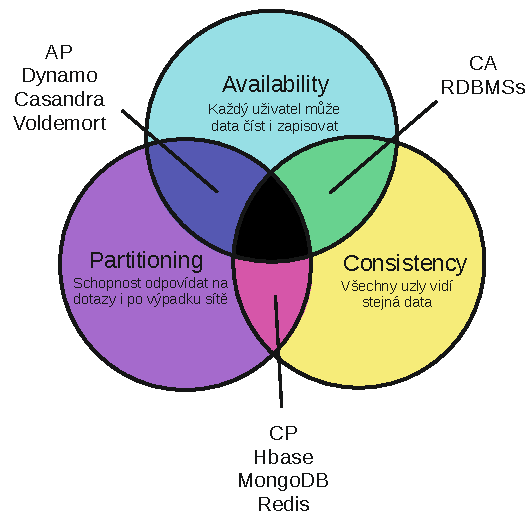
\includegraphics[width=0.7\textwidth, angle=0]			{files/cap}
	\caption[CAP teorém]{CAP teorém}\label{fig:cap}
\end{figure}
\pagebreak
\subsubsection{Typy NoSQL databází}
Mezi NoSQL databáze se řadí především zástupci těchto skupin:
\paragraph{Key-value databáze}
Databáze typu key-value fungují na velmi jednoduchém datovém modelu. Jedná se o množinu párů, kdy je každý prát tvořen unikátním klíčem a libovolně strukturovanou hodnotou. Vyhledávání je pak možné pouze podle daného klíče. Z jednoduchého modelu vychází i velmi jednoduchá funkcionalita ale naopak velká výkonost při čtení a zápisu velkého množství dat.
\begin{description}
	\item[Významní zástupci: ] DynamoDB, BerkleyDB, Redis, Riak
\end{description}

\paragraph{Dokumentově orientované databáze}
Tento typ DBMS logicky navazuje na key-value databáze. Základním prvkem je dokument opatřený unikátnm identifikátorem. Oproti key-value databázím bývají robustnější a některé umožňují například extrahovat metadata z uložených dokumnetů. Jako data v těchto databázích jsou ukládány především soubory ve formátech HTML, XML, JSON, PDF a další
\begin{description}
	\item[Významní zástupci: ] MongoDB, CouchDB, MarkLogic, RavenDB
\end{description}

\paragraph{Objektově orientované databáze}
V těchto databázích se jednotlivé záznamy  reprezentují jako instance tříd.  Celkově tento přístup kopíruje vlastnosti objektově orientovaného programování jako je zapouzdření či přetěžování. Výhoda těchto databází je v tom, že jsou záznamy uložené ve stejné podobě jako jsou definovány v rámci programu, který je zpracovává, což svyšuje prezistenci dat.
\begin{description}
	\item[Významní zástupci: ] ObjectDB, Db4o
\end{description}

\paragraph{Grafové databáze}
Jedná se o databáze založeny na teorii grafů. Jednotlivé prvky jsou ukládány do grafové struktury, které je složena z vrcholů a hran, kde vrcholy reprezentují  jednotlivé prvky a hrany modelují vztahy mezi nimi.
\begin{description}
	\item[Významní zástupci: ] NEO4J, HyperGraphDB, Infogrid
\end{description}

\paragraph{Sloupcově orientované databáze}
Jsou jedním z představitelů NoSQL databází. Vyznačují se především tím, že data ukládají ve sloupcové formě, narozdíl od relačních databází, které ukládají data do řádků. Hlavním představitelem sloupcových databází je databáze HBase. Jejímu detailnímu popisu se budou věnovat následující kapitoly.
\begin{description}
	\item[Další významní zástupci: ] BigTable, Cassandra, HyperTable
\end{description}

\section{Distribuované výpočty}
Jednoduše řečeno se jedná o přístup, kdy rozdělíme velký komplikovaný výpočet na více menších a jednodušších úloh a tyto úlohy pak provedeme paralelně na více výpočetních uzlech. Hlavní motivace k tomuto jednání je především rychlejší zpracování výsledku. Jedním z možných typů distribuovaných výpočtů je i paradigma Mapreduce. 

\subsection{MapReduce}
MapReduce je programovací paradigma určené k provádění výpočtů, které by za normálních okolností trvaly značné množství času a to zejména z důvodů velkého množství dat. Tyto výpočty se pak snaží dokončit v přijatelném časovém horizontu. Princip byl poprvé představen v roce 2004 v  práci pro firmu Google jako jedno z opatření pro zvládání obrovského množství dat, se kterým se museli potýkat.

V MapReduce jsou data modelována do párů klíč/hodnota. Tento formát je velmi jednoduchý, přesto se dají téměř všechny údaje takto prezentovat. Tato jednoduchá datová struktura tak umožňuje snadné zpracování dat efektivním způsobem. Klíč a hodnota může být cokoliv. Může se jednat o řetězce, čísla nebo komplexní struktury.

Mapreduce se skládá ze dvou hlavních fází, mapovací fáze a redukční fáze. Nejdříve je spuštěna mapovací funkce, která je dále spočtena nad jednotlivými prvky z množiny uspořádaných dvojic (klíč, hodnota), jež produkuje přechodné klíče a hodnoty.\cite{HadoopDG}
Poté jsou všechny tyto přechodné hodnoty asociované se stejným klíčem seskupeny a následně poslány se do redukční fáze. Redukční fáze přijme na vstupu klíč a související množinu hodnot. Jako výstup je pak množina uspořádaných dvojic, která splňuje zadaná kritéria.
\begin{figure}[h]\centering
	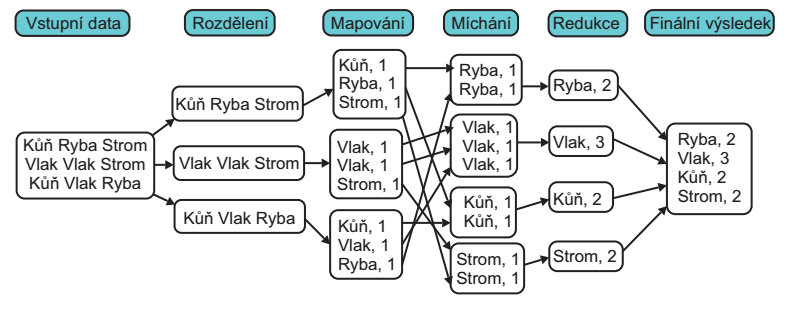
\includegraphics[width=1\textwidth, angle=0]			{files/MapReduce}
	\caption[Diagram MapReduce procesu]{Diagram MapReduce procesu}\label{fig:mapred}
\end{figure} 

Jak vstupní data, tak mezivýsledky i finální výsledky jsou ve formátu klíč/hodnota. Jak je vidět na obrázku \ref{fig:mapred} probíhají mapovací a redukční fáze paralelně. Z diagramu je také zřejmé, že mezi mapovací fází a fází míchání(shuffling) dochází k přenosu průběžných výsledků mezi jednotlivými výpočetními uzly. Právě optimalizací přesunů v těchto místech se bude zabývat hlavní část této práce. 
MapReduce je také často popisována funkcí: 

\begin{eqnarray}
	map: (k_1, v_1) \rightarrow  list(k_2, v_2) \nonumber \\
	reduce: (k_2, list(v_2)) \rightarrow list(k_3, v_3) \nonumber 
\end{eqnarray}



\chapter{Současný stav a použité technologie}
V této úvodní kapitole je dán prostor pro seznámení se s technologiemi a projekty, se kterými se bude buď přímo pracovat nebo je jejich znalost pro pochopení problematiky nezbytná. Jako první je představen projekt Hadoop\textsuperscript{TM}, který je vyvíjen pod záštitou Apache\textsuperscript{TM} foundation jako celek. Vše, co bude v této práci představeno, se bude odehrávat v rámci tohoto takzvaného ekosystému. Po uvedení celého Hadoopu jsou detailněji uvedeny produkty, které jsou součástí tohoto ekosystému a se kterými se bude dále pracovat. Jedná se především o databázový systém HBase a také souborový systém HDFS, který je v celém modelu používán. Mimo to je pak zde uvedena ukázka kódu pro typický příklad MapReduce úlohy s postupným popisem zpracování. Na závěr je uvedena trocha teorie o dělení hypergrafů, jelikož tento problém bude hrát klíčovou roli v celkovém řešení.


\section{Hadoop Ekosystém}
Apache Hadoop je platforma která zastřešuje projekty vyvíjející software pro spolehlivé, škálovatelné a paralelní zpracování dat na počítačových clusterech. Je založen na dvou stěžejních  technologiích pocházejících od firmy Google  a to na distribuovaném souborovém systému Google File System (GFS)\cite{GFS} a na algoritmu MapReduce\cite{HadoopDum}. Všechny klíčové projekty v systému Hadoop jsou sdruženy pod Apache Software foundation, která poskytuje podporu pro tyto projekty. Jedná se o open-source software a všechny komponenty jsou psány v programu Java.

\subsection{Základní principy}
Podstata Hadoopu spočívá v uložení dat na velkém množství výpočetních úzlů spojených do clusterů. Většinou se jedná o běžný hardware. Na těchto uzlech jsou data uložená ve vlastním souborovém Systému HDFS. K výpočtům nad clusterem se využívá princip Mapreduce, který bude osvětlen v následující kapitole. Systém Hadoop je charakteristický především následujícími vlastnostmi, které ho odlišují od klasických databázových systémů.

\begin{description}

  \item[Horizontální škálovatelnost a komoditní hardware] \hfill \\
  Pro objemy dat, jimiž by se měl Hadoop při svém zpracovávání primárně zabývat, je poměrně složité a především velmi drahé dosáhnout dostatečné škálovatelnosti pomocí vertikálního škálování, tedy přidávání výkonu a zdrojů ke stávajícím výpočetním uzlům. Proto Hadoop využívá horizontálního škálování. Díky horizontálnímu škálování se nabízí využití komoditního hardwaru namísto specializovaných výpočetních uzlů. Systém tedy běží na velkém množství samostatných počítačů spojených do clusteru.
  \item[Řešení selhání hardwaru] \hfill \\
   S předchozím bodem úzce souvisí řešení případných výpadků jednotlivých uzlů. Kvůli velkému počtu výpočetních uzlů a díky použití běžného hardware jsou výpadky poměrně časté. Hadoop je ale navržen tak, že se nesnaží tyto výpadky minimalizovat, ale počítá s nimi. Data jsou dostatečně replikovány a pokud dojde k výpadku při zpracování dat, je přerušená úloha provedena na jiném uzlu obsahující danou replikaci a zároveň je automaticky vytvořena nová záloha dat. Defaultně je zálohovací faktor nastaven na {\texttt{3}} , tedy každý soubor je uložen ve třech kopiích na různých výpočetních uzlech.  
  \item[Přenášení kodů k datům] \hfill \\
  Kvůli velkým objemům dat a poměrně nízké propustnosti sítě spojující jednoltivé výpočetní uzly v clusteru je velmi výhodné namísto rozesílání dat na jednotlivé výpočetní uzly rozesílat na ně pouze kód výpočtu a minimalizovat tak přesuny dat mezi uzly. Na každém uzlu je tak vykonán výpočet pokud možno s lokálními daty.
  \item[Abstrakce od distribuovaných a paralelních aplikací] \hfill \\
  Hadoop se snaží co nejvíce odstínit vývojáře Hadoop aplikací od řešení zpracování pomocí paralelního a distribučního zpracovaní. Proto poskytuje poměrně jednoduché a dobře definované rozhraní pro jednotlivé komponenty. Při práci s těmito rozhraními tak není nutné řešit, jak se bude kód v clusteru distrubuovat ani další záležitosti spojené s paralelním zpracováním a dovoluje se zaměřit na business logiku aplikace. Cenou za toto zjednodušení je pak právě omezené rozhraní bez možnosti detailnějšího nastavení. 

\end{description}


\clearpage
\subsection{Hadoop Ekosystém}
Následující kapitola je určena k seznámení s ekosystémem Hadoop, který kromě základních modulů MapReduce a HDFS obsahuje množství dalších modulů. Složení ekosystému se ale liší v závislosti na konkrétní distribuci používaného systému Hadoop. Je sice možné zvolit si tyto aplikace podle svého výběru a využít přímo zdroje od firmy Apache, ale v praxi se využívají spíše již částečně nakonfigurované distribuce, které navíc nabízejí i možnost placené podpory. Mezi největší hráče na trhu patří distribuce od firem Cloudera, MapR a Hortonworks.\cite{CLOUDERA} Pro účely této práce byla vybrána distribuce Cloudera, protože se jedná o open-source projekt a také kvůli největšímu podílu na trhu.Náhled na celý ekosystém je zobrazen na obrázku.\ref{fig:eko} V následujícím výpisu se nachází hlavní moduly, které jsou obsaženy ve většině distribucí.

\begin{figure}[h]\centering
	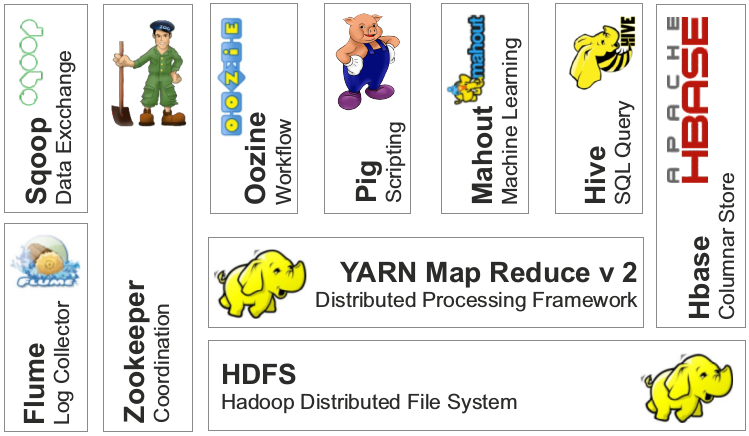
\includegraphics[width=1\textwidth, angle=0]{files/HadoopEco}
	\caption[Hadoop Ekosystém]{Hadoop Ekosystém}\label{fig:eko}
\end{figure}

\paragraph{Nástroje pro vývoj}
\begin{description}
\item[YARN] \hfill \\
YARN je klíčovým prvkem Hadoop 2. Někdy je také zvaný  MapReduce v2. Jedná se o distribuovaný operační systém, který odděluje řízení zdrojů a řízení kapacit od zpracovávající komponenty. To umožňuje  podporovat větší škálu přístupů ke zpracování dat a širší pole aplikací.

\item[Hive] \hfill \\
Hive umožňuje dotazování nad velkými datasety uloženými v distribuovaném systému a také jejich řízení. Poskytuje mechanismus k vytvoření struktury nad těmito daty a následně nad daty provádět dotazy v SQL-like  jazyku HiveQL. Kromě toho umožňuje také využití klasického map/reduce postupu v případech, kdy není výhodné použít HiveQL. 

\item[Pig] \hfill \\
Pig poskytuje prostředí pro zpracování jednoduchého skriptovacího jazyka Pig Latin, ve kterém je přeložen na sérii MapReduce úloh. Pig Latin abstrahuje od MapReduce schématu a nabízí dotazování na vyšší úrovni, podobné jako SQL.

\item[Mahout] \hfill \\
Mahout je škálovatelná knihovna pro strojové učení. Jsou v ní implementovány algoritmy pro clustering, klasifikaci a kolaborativního filtrování optimalizované pro běh v prostředí Hadoopu.
\end{description}
\paragraph{Ukládání dat a správa metadat}
\begin{description}
\item[HDFS] \hfill \\
Jedná se o distribuovaný souborový systém navržený  pro provoz na komoditním hardwaru ve velkých datových skladech, souborový systém HDFS bude detailněji představen v následující kapitole.

\item[HBase] \hfill \\
Hbase je sloupcově orientovaný databázový systém, který běží nad HDFS. Nepodporuje strukturovaný dotazovací jazyk a poskytuje prakticky pouze CRUD operace. HBase bude stejně jako HDFS představen detailněji v následujících kapitolách.
\end{description}
\paragraph{Nástroje pro řízení}
\begin{description}
\item[ZooKeeper] \hfill \\
Poskytuje provozní služby pro Hadoop cluster. Jedná se o distribuované konfigurační, synchronizační služby a o jmenné registry pro distribuovaný systém. 

\item[Oozie] \hfill \\
Aplikace používaná pro plánování Hadoop úloh. Je složena ze dvou hlavních částí. V první části se ukládají a spouštějí různé typy hadoop úloh (Mapreduce, Pig, Hive, atd.) a z části, která koordinuje běh daných úloh na základě předdefinovaných plánů a dostupnosti dat.
\end{description}

\paragraph{Získávání a agregace dat}
\begin{description}
\item[Sqoop] \hfill \\
Nástroj sloužící k efektivnímu přenosu dat z relačních databází do Hadoopu k dalšímu zpracování. Zpracovat tyto data pak může buď MapReduce úloha nebo jiný nástroj (Hive, Pig). Je také možné data vložit do HBase databáze.
\item[Flume] \hfill \\
Služba pro efektivní získávání, agregování a přesouvání velkého množství streamovaných dat do HDFS. Typicky se používá k ukládání logů z jednoho zdroje (webové logy, bankovní logy) a agreguje je v HDFS pro pozdější zpracování.
\end{description}

\section{MapReduce v Hadoopu}
Jak funguje MapReduce na Hadoopu bude demonstorváno na následujícím příkladě WordCount. Je to jednoduchá úloha, kde jak již název napovídá, je úkolem zjistit četnost slov nacházejících se v textu. Tato ukázková úloha je dostuná v oficiálním tutorialu na webových stránkách Cloudery \footnote{\texttt{http://www.cloudera.com/content/cloudera/en/documentation/hadoop-tutorial /CDH5/Hadoop-Tutorial/}}, kde jsou uvedeny i pokročilejší metody pro řešení těchto úloh. Uvažujme, že zpracováváme dva soubory, první obsahující text "Hello World Bye World"  druhý pak "Hello Hadoop Goodbye Hadoop".
\begin{enumerate}
\item Implementace třídy Mapper pomocí metody Map zpracovává po jedné řádce dat ve formátu TextInputFormat. Každou řádku poté rozdělí pedle mezer na tokeny pomocí metody StringTokenizer a emituje key-value pár <Hello, 1>.
\item pro první soubor emituje map funkce <Hello, 1> <World, 1> <Bye, 1> <World, 1>
\item pro druhý to je <Hello, 1> <Hadoop, 1> <Goodbye, 1> <Hadoop, 1>
\item WordCount obsahuje i combiner. Výstup každé map funkce projde skrz lokální combiner (stejný jako v Reduceru) a po seřazení  klíčů provede lokální agregaci dat
\item výstup první map funkce: <Bye, 1> <Hello, 1> <World, 2>
\item výstup druhé map funkce  <Goodbye, 1> <Hadoop, 2> <Hello, 1>
\item Implementace Reducer třídy pomocí metody reduce sečte hodnoty pro stejné klíče
\item výstup Hadoop jobu pak je <Bye, 1> <Goodbye, 1> <Hadoop, 2> <Hello, 2> <World, 2>
\end{enumerate}
\pagebreak
\begin{lstlisting}[frame=single]  % Start your code-block


public class WordCount {

  public static class Map extends MapReduceBase implements Mapper<LongWritable, Text, Text, IntWritable> {
    private final static IntWritable one = new IntWritable(1);
    private Text word = new Text();

    public void map(LongWritable key, Text value, OutputCollector<Text, IntWritable> output, Reporter reporter) throws IOException {
      String line = value.toString();
      StringTokenizer tokenizer = new StringTokenizer(line);
      while (tokenizer.hasMoreTokens()) {
        word.set(tokenizer.nextToken());
        output.collect(word, one);
      }
    }
  }

  public static class Reduce extends MapReduceBase implements Reducer<Text, IntWritable, Text, IntWritable> {
    public void reduce(Text key, Iterator<IntWritable> values, OutputCollector<Text, IntWritable> output, Reporter reporter) throws IOException {
      int sum = 0;
      while (values.hasNext()) {
        sum += values.next().get();
      }
      output.collect(key, new IntWritable(sum));
    }
  }

  public static void main(String[] args) throws Exception {
    JobConf conf = new JobConf(WordCount.class);
    conf.setJobName("wordcount");
    conf.setOutputKeyClass(Text.class);
    conf.setOutputValueClass(IntWritable.class);
    conf.setMapperClass(Map.class);
    conf.setCombinerClass(Reduce.class);
    conf.setReducerClass(Reduce.class);
    conf.setInputFormat(TextInputFormat.class);
    conf.setOutputFormat(TextOutputFormat.class);
    FileInputFormat.setInputPaths(conf, new Path(args[0]));
    FileOutputFormat.setOutputPath(conf, new Path(args[1]));
    JobClient.runJob(conf);
  }
}
\end{lstlisting}

\section{HDFS}
Hadoop Distributed File Systém (HDFS) nabízí způsob skladování velkých souborů na více samostatných počítačích, který je rozdílný oproti klasickému přístupu skladování dat na jednom stroji s dostatečnou diskovou kapacitou. HDFS je navržen na základech Google File Systemu (GFS) a běží na nativním filesystému (Ext3, Ext4,XFS). HDFS je určen pro skladování především velkých souborů (100 MB a více) v menším počtu (řádově miliony) a k ukládání streamovaných dat. Systém dále není vhodný pro soubory, u nichž se očekává časté upravování, a to protože je možné připisovat data pouze na konec souboru. Systém je odolný proti chybám v replikaci a výpadkům v distribuci dat.\cite{HDFSWEB}

\begin{figure}[h]\centering
	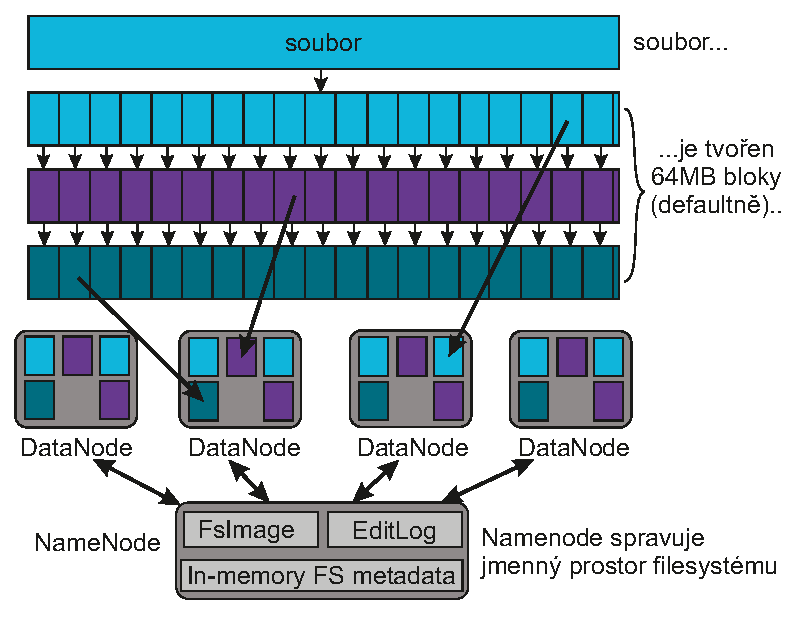
\includegraphics[width=0.8\textwidth, angle=0]{files/hdfs}
	\caption[Diagram uložení souboru v systému HDFS]{Diagram uložení souboru v systému HDFS}\label{fig:hdfs}
\end{figure}

HDFS umožňuje, stejně jako většina běžných souborových systémů, operace čtení, zápisu a mazání souborů a vytváření a mazání adresářů. Vždy, když je načten nový soubor do HDFS, je zreplikován do žádoucího počtu, který určuje replikační faktor (defaultní hodnota je 3) a rozdělen do bloků dat o fixní délce (defaultně 64MB). Tyto bloky jsou pak rozdistribuovány a uloženy  ve vybraných uzlech clusteru určených pro skladování, tzv. DataNodes viz.\ref{fig:hdfs} . V HDFS se informace o souborech neukládají společně s daty, ale jsou uloženy na vyhrazeném serveru nazývaném NameNode. Při přístupu k datům klient nejdříve zadá požadavek na data na NameNode, který následně vrátí adresy databloků s požadovanými daty. NameNode tedy přímo nemanipuluje s daty.

NameNode uchovává a poskytuje strom jmenného prostoru a adresy fyzického umístění bloků ve své operační paměti. Dále ukládá perzistentní záznam těchto adres (kontrolní bod) a registr modifikací (žurnál) pro zotavení z havárie v nativním systému souborů hostitelského počítače. HDFS umožňuje i  vytvoření kopie kontrolního bodu a žurnálu na další výpočetní uzel nazývaný SecondaryNameNode. Ten pak slouží jako záloha dat serveru NameNode  (nenahrazuje tedy funkci primárního NameNode v případě výpadku, pouze poskytuje data pro jeho obnovu). Ve verzi Hadoop 2+ je už možné mít Standby NameNode, který v případě výpadků může primární NameNode plně a okamžitě nahradit. 

Přistupovat k HDFS je možné přímo a to přes nativního klienta nebo pomocí Java nebo C++ API. Dále je možný přístup přes proxy server podporující REST, Thirft a Avro server.

\section{HBase}
Jedná se o sloupcově orientovanou databázi, někdy označovanou jako Hadoop databáze. HBase podporuje náhodné real-time CRUD operace (narozdíl od HDFS). Je primárně navržená pro uchovávání velkých tabulek o miliardách řádků a milionech sloupcích a jedná se o NoSQL databázi. Nepodporuje tedy přístup založený na SQL jazycích ani relační model. Stejně jako HDFS se vyznačuje jednoduchým klientem a Java API. HBase je založena na projektu BigTable od firmy Google\cite{BigTable} a stejně jako byl BigTable postaven nad GFS je HBase postavena nad HDFS.\cite{HbaseDG}

HBase nebyla zavedena za účelem nahrazení klasických RDBMS a ani k tomuto účelu není využívána. HBase je výhodné použít, jak již bylo řečeno, v případě rozsáhlých tabulek. Výborné výsledky vykazuje při vykonávání jednotlivého náhodného výběru z databáze a při vyhledávání dle klíče. Hbase je také vhodným řešením v případě, že jednotlivé řádky tabulky jsou velmi různorodé a v případě řidkých databází, kdy je velký počet sloupců a většina z nich obsahuje nulovou hodnotu. Nevhodné využití je pak právě pro suplování úloh pro tradiční RDBMs jako jsou transakční aplikace nebo relační analýza.\cite{HBaseWEB}

\subsection{Data model HBase}


Data v databázi HBase jsou uložena v tabulkách. Jednotlivé tabulky obsahují řádky. Na každý řádek odkazuje unikátní klíč. Jako hodnota klíče se bere bitové pole. Klíč u HBase tedy může být cokoli, string, long nebo vlastní datová struktura. Každý řádek je složen ze sloupců, které jsou sdruženy do rodin (column families). Tyto rodiny sloupců jsou definovány staticky při vytváření databáze narozdíl od samotných sloupců, které se mohou přidávat libovolně. Data jako taková jsou pak uložena v buňkách. Tyto buňky jsou identifikovány pomocí řádku, rodiny, sloupce a časovou značkou(timestamp). Obsah každé buňky je pak uchováván také jako pole bitů. Data v buňkách jsou navíc verzovány. Každá buňka defaultně uchovává poslední tři zadané hodnoty s tím, že pokud není v dotazu specifikována konkrétní verze, vrací vždy tu nejmladší. Řádky jsou v každé tabulce seřazeny lexikograficky podle svého klíče. Příklad takové tabulky je uveden v obrázku \ref{fig:hbase}.

\begin{figure}[h]\centering
	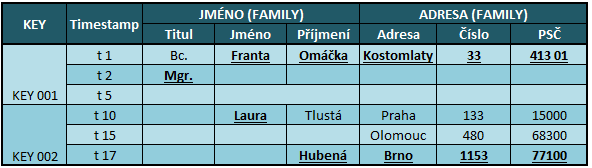
\includegraphics[width=0.8\textwidth, angle=0]{files/hbase}
	\caption[Datový model HBase]{Datový model HBase}\label{fig:hbase}
\end{figure}

\subsection{HBase Architektura}
HBase je distribuovaná databáze. Proto je i architektura složitější než u databází běžících na jednom výpočetním uzlu. HBase musí řešit všechny problémy typické pro distribuované aplikace jako je koordinace a řízení vzdálených procesů, blokování, distribuce dat a příliš velká síťová komunikace. HBase však k tomuto z velké části využívá služeb v rámci Hadoop a Zookeeper. Následující obrázek \ref{fig:hbasearch} popisuje hlavní architektonické komponenty HBase.
\begin{figure}[h]\centering
	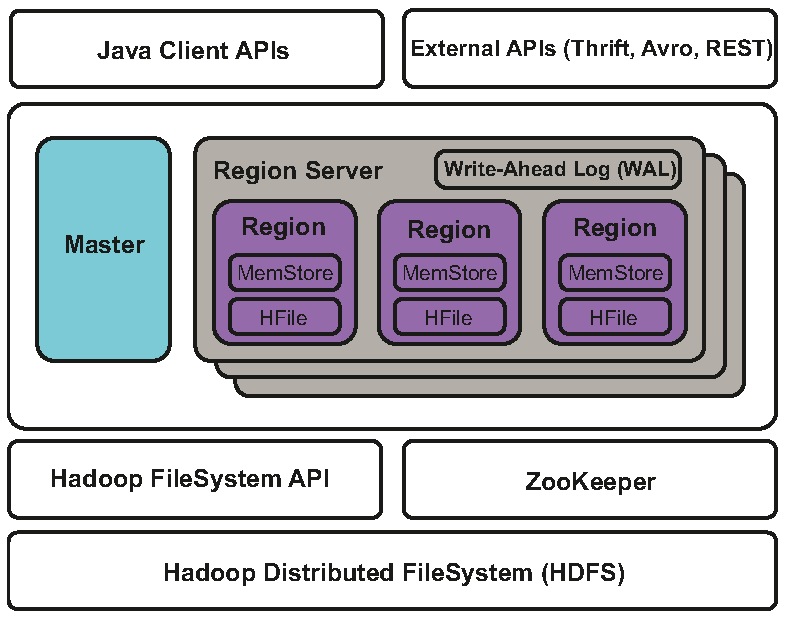
\includegraphics[width=0.8\textwidth, angle=0]{files/hbase-architecture}
	\caption[Architektura databáze HBase]{Architektura databáze HBase}\label{fig:hbasearch}
\end{figure}

Jednotlivé tabulky jsou složeny z regionů. Region je vždy určitý rozsah řádků uložený pohromadě. Protože jsou řádky v databázi ukládány v lexikografickém pořádí, je nutné počítat s tím, že se velikost těchto rozsahů, tedy regionů, bude v čase měnit. Proto se v případě, kdy velikost regionu překročí stanovenou hranici, rozdělí region na dva přesně v půli podle prostředního klíče. Naopak v případě, kdy se regiony příliš zmenší, dojde k jejich sloučení. Regiony jsou uložené v region serverech. Každý region server může obsahovat jeden a více regionů. Region je však vždy jen na jednom serveru. Master server je zodpovědný za správu region serverů. Pro koordinaci se využívá Zookeeper. Na každém regionu je uložen určitý rozsah klíčů. Rozdělení dat do region serverů umožňuje rychlou obnovu v případě pádu region serveru a také ulehčuje load balancing pokud dochází k přetěžování některých serverů. Všechny tyto činnosti včetně rozdělování velkých regionů jsou prováděny automaticky bez zásahu uživatele.

\subsection{Architektura uložiště RDBMS vs HBase}
Dříve než bude uveden detailní pohled na uložení dat v databázi HBase, je na místě popsat základní rozdíl mezi typickou architekturou uložení dat v RDBMS a v HBase. Typické RDBMS ukládá data do struktury B+ Trees oproti tomu HBase a ostatní Big Table architektury využívají Log-Structured Merge Trees\cite{hbase2011}.

\subsubsection{B+ Trees}
Jedná se o stromovou datovou strukturu, která vychází z B-stromu. Umožňuje rychlé vkládání, vyhledávání a mazání dat. Záznamy v tabulkách jsou identifikovány za pomoci klíčů. Všechny hodnoty jsou uloženy jen na listech stromu, oproti klíčům, které jsou uloženy i ve vnitřních uzlech. V implementaci těchto stromů se přidává do všech listů kromě vlastních klíčů i odkaz na následujícího sourozence.\cite{efi} To umožňuje velmi efektivní sekvenční prohledávání aniž by výrazněji stoupla paměťová náročnost na uložení stromu, odkaz na sourozence je v obrázku znázorněn červenými políčky \ref{fig:btree}. 

V B+stromech je data-locality dosažená na úrovni stránek, kde stránky odpovídají blokům v jiných systémech. Stránka tak může vypadat například takto:
\begin{itemize}
	\item Odkaz na předchozí stránku
	\item Odkaz na následující stránku
	\item key: A $\rightarrow d_A$
	\item key: B $\rightarrow d_B$
	\item key: C $\rightarrow d_C$
	\item key: D $\rightarrow d_D$
\end{itemize}

Vždy, když se vkládá nový záznam, doplní se daná stránka požadovaným záznamem. Pokud dojde k případu, že stránka už je plná, rozdělí se na 2 poloprázdné stránky a upraví se patřičně rodič těchto stránek. Tímto dochází k fragmentaci dat na disku, když jednotlivé logicky sousedící stránky neleží vedle sebe fyzicky.
\begin{figure}\centering
	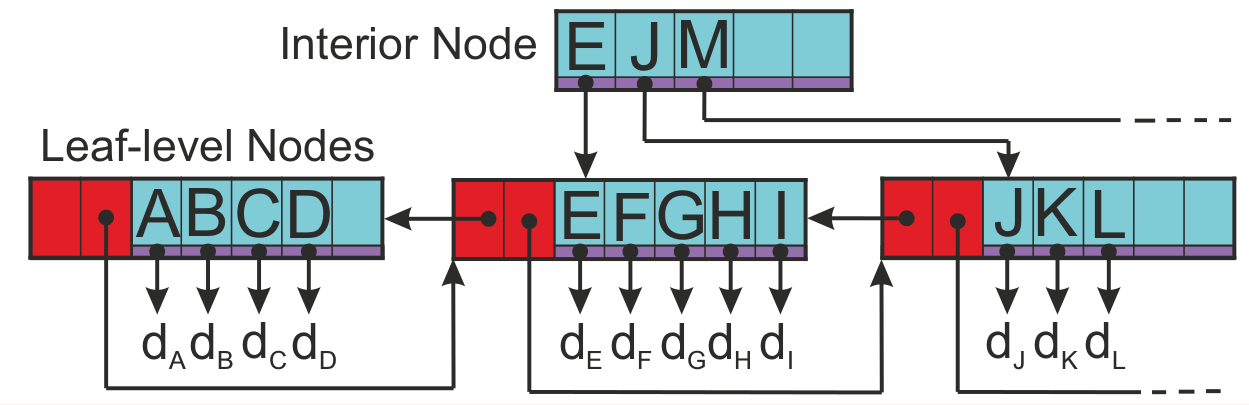
\includegraphics[width=0.7\textwidth, angle=0]{files/Bplustree}
	\caption[Příklad B+ stromu.]{Příklad B+ stromu. Obsahuje data $d_1$ až $d_7$}\label{fig:btree}
\end{figure}


\subsubsection{Log-Structured Merge Trees}
Log-Structured Merge Trees využívají způsob odlišný od B+ stromů. Všechny příchozí data jsou nejprve ukládány v logovacích souborech a to kompletně sekvenčně. Jakmile jsou informace uložené v logu, uloží se data v in-memory uložišti, kde jsou uloženy naposledy upravené záznamy. Vždy, když je k dispozici dostatečný počet záznamů, dojde k zapsání už seřazených dat do uložiště souborů. Po zapsání dat na disk je log soubor smazán. 


Datové soubory jsou pak strukturovány podobně jako B stromy, s tím že jsou optimalizovány pro sekvenční přístup na disku. Všechny uzly stromu jsou zaplněny a uloženy v sigle-page nebo multi-page bloku. Při přidávání dat se uložená data na disku v multi-page blocích spojí s příchozími in-memory daty. Tento proces je znázorněn na obrázku \ref{fig:lms}.  Vždy, když data využijí celou kapacitu bloků, dojde k vytvoření nového.
Postupně se tak zvyšuje počet vytvořených souborů. Tyto soubory jsou pak spojovány do větších celků. Všechny tyto soubory jsou uloženy sekvenčně za sebou a tak je umožněn optimální sekvenční přístup k datům.
Strom může být také rozdělen v případě, kdy je potřeba vložit nová data s klíči mezi ostatními.
Mazání záznamů se provádí dávkově. Každý záznam, který je určený ke smazání je označen jako smazaný, a při nahlížení do dat se ignoruje. Při přepisování stránek pak dojde k odstranění těchto záznamů ze stromu.

Z těchto rozdílných přístupů k uložení dat vyplývá, že B+ stromy jsou určeny pro úlohy, kde se očekává častá modifikace již vložených dat, zatímco LSM stromy jsou určeny k ukládání velkého množství dat a jeho následovnému čtení.


\begin{figure}\centering
	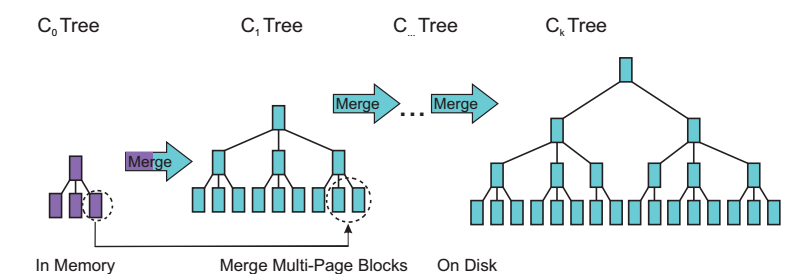
\includegraphics[width=1\textwidth, angle=0]{files/lms}
	\caption[Iterativní Merge Multi-Page bloků v LMS stromu ]{Iterativní Merge Multi-Page bloků v LMS stromu }\label{fig:lms}
\end{figure}

\subsection{Fyzické uložení dat}	
Pro většinu uživatelů je forma fyzického uložení dat v HBase zcela skrytá a k plnohodnotnému využívání databáze prakticky nevýznamná. Avšak pro potřeby této práce, je nezbytné tuto část osvětlit více, než je zapotřebí pro běžné využívání. Na obrázku \ref{fig:hbasehdfs} je znázorněno schéma uložení dat, které zobrazuje uložení dat v souborovém systému HDFS. Hbase pracuje především se dvěma hlavními typy souborů. Se soubory HLog reprezentující write-ahead log (WAL) a HFile pro uložení dat.\cite{hbasecon}

\begin{figure}[h]\centering
	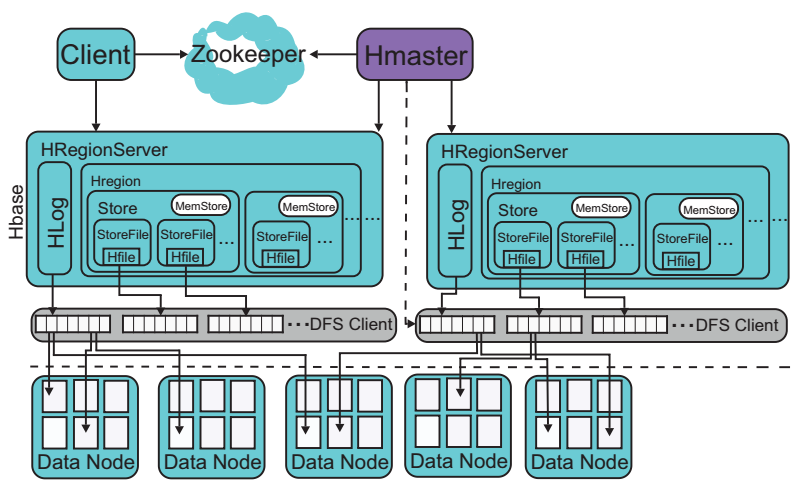
\includegraphics[width=1\textwidth, angle=0]{files/HBaseHDFS}
	\caption[Schéma ukládání dat z HBase v HDFS]{Schéma ukládání dat z HBase v HDFS}\label{fig:hbasehdfs}
\end{figure}

\subsubsection{Formát HFile}
Formát souboru HFile je navržen tak, aby ukládal data co nejefektivněji. Je založen na formátu souboru TFile z Hadoopu. Soubor obsahuje několik bloků, jak je vidět na obrázku \ref{fig:hfile}, z nichž jsou fixní pouze info a trailer bloky. Tyto bloky jsou uloženy na konci souboru a ukončují tak daný soubor, který se stává neměnným. V index blocích jsou uloženy offsety data a metadata bloků. Jak metadata bloky tak i data bloky jsou nepovinné, nicméně už z podstaty věci jsou data bloky téměř vždy součástí Hfile souboru. Velikost jednotlivých bloků je defaultně definována na 64 KB. Je možné tuto velikost změnit v závislosti na očekávané struktuře dotazů na databázi. Čím větší bloky, tím efektivnější bude sekvenční prohledávání databáze, naopak náhodný přístup bude efektivní méně. V jednotlivých blocích se sekvenčně ukládají KeyValue instance v KeyValue formátu. Velikost bloků není fixní, odvíjí se od velikosti poslední vložené key value instance, která se do bloku uloží celá a pak teprve dojde k uzavření bloku. V praxi tedy boky bývají o něco větší než je definovaná hodnota. Je možné také použít libovolný komprimační algoritmus na ukládaná data, což ale neovlivní celý proces, protože checksum je dopočítáván až po přidání poslední key value instance.
\begin{figure}[h]\centering
	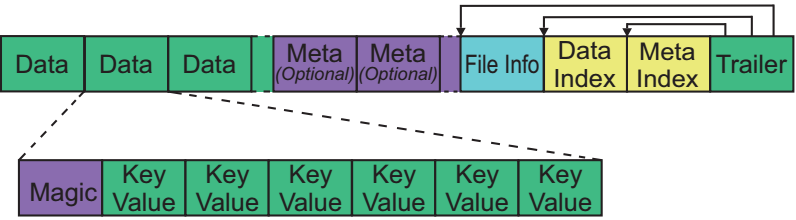
\includegraphics[width=0.8\textwidth, angle=0]{files/HFile}
	\caption[Formát souboru HFile]{Formát souboru HFile}\label{fig:hfile}
\end{figure}


Ačkoli se nabízí myšlenka, že velikost bloků v HFile nastavená na 64KB souvisí s velikostí souborů v HDFS, který je nastaven na 64 MB, není mezi těmito hodnotami žádná spojitost. HFile jsou v HBase ukládány jako běžné soubory a HDFS je vnímá pouze jako binární data. Na obrázku \ref{fig:hfiletohdfs} je zobrazeno schéma ukládání HFile souborů do HDFS.

\begin{figure}[h]\centering
	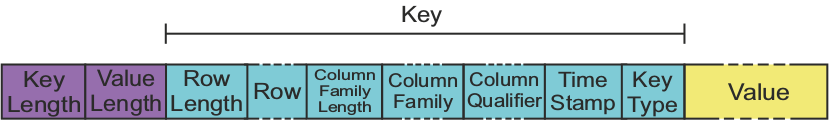
\includegraphics[width=1\textwidth, angle=0]{files/key-value}
	\caption[Formát KeyValue struktury]{Formát KeyValue struktury}\label{fig:keyvalue}
\end{figure}



\paragraph{Formát KeyValue}
KeyValue je struktura, která reprezentuje fyzické uložení jedné buňky z tabulky. Z obrázku \ref{fig:keyvalue} vyplývá, že jako část klíče se používá mimo jiné  název tabulky, family a sloupce. Tento klíč se vyskytuje u každé buňky a proto se doporučuje, mít vše pojménováno co nejkratšími identifikátory.	
\begin{figure}[h]\centering
	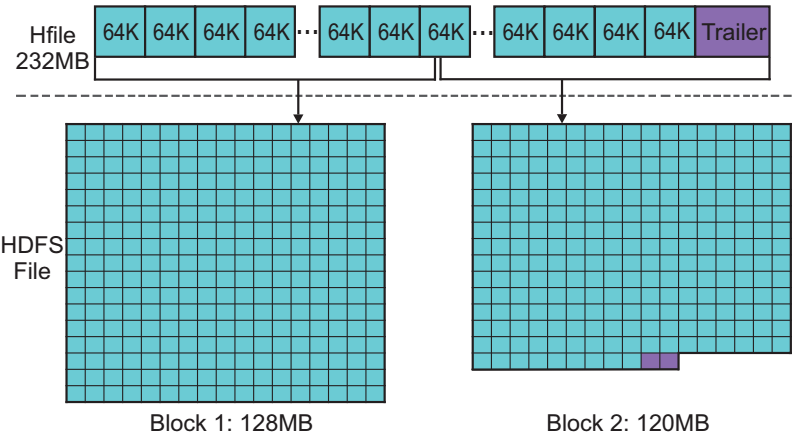
\includegraphics[width=0.8\textwidth, angle=0]{files/HFileToHDFS}
	\caption[Rozložení Hfile do bloků dat v HDFS]{Rozložení Hfile do bloků dat v HDFS}\label{fig:hfiletohdfs}
\end{figure}


\subsubsection{Write-Ahead Log}
Region servery ukládají příchozí data do paměti, do doby něž se jich nahromadí dostatečné množství a poté je najednou zapíše na disk. Ve fázi, kdy se data hromadí v paměti, jsou ale zranitelná a v případě výpadku dojde k jejich ztrátě. Právě pro zamezení tohoto problému se používá WAL. Jeho funkce tedy je omezit dopady výpadku. Do logu se proto zapisují všechny změny dat, a až v případě, že jsou úspěšně uloženy na disk, je klient informován o úspěšném uložení dat. 

\section{HyperGraph Partitioning}
Hypergraph partitioning je známý problém, řešený hlavně při návrhu rozložení VLSI (Very-large-scale integration). Obecně lze říci že se jedná o operaci, která má za cíl rozdělit hypergraf do dvou nebo zhruba stejně velkých částí tak, aby při oddělování bylo přerušeno co nejméně hran spojující jednotlivé uzly v grafu.

Pro řešení problému dělení grafů a hypergrafů se používají především heuristiky založené na algoritmu Kernighan-Lin (KL). Především díky rychlosti běhu a poměrně dobrým výsledkům. KL algoritmus je navržen průvodně pro bipartitioning grafů. Na jeho základech však vznikla většina pokročilejších algoritmů pro dělení grafů. KL algoritmus začíná počátečním rozdělením na dvě části, následně provede určitý počet kroků, dokud se nenajde lokální minimum bipartitity. Každý krok obsahuje sekvenci prohození vrcholů. Stejnou strategii prohazování vrcholů při řešení problému dělení hypergrafů použili Schweikert-Kernighan\cite{graph1}. Fiduccia-Mattheyses\cite{graph2} uvedli rychlejší implementaci KL algoritmu pro dělení hypergrafů. Byla založená na nahrazení vyměňování uzlů za jejich přesouvání.  V kombinaci s použitím správných datových struktur výrazně klesla časová náročnost algoritmu. Na těchto základech a mnoha dalších poznatcích je pak vyvinut nástroj PaToH (PaToH:Partitioning Tools for Hypergraphs), který bude využit právě pro řešení dělení hypergrafu v implementační části této práce.

\subsection{Definice problému}
Hypergraf $H=(V,N)$ je definován jako množina vrcholů $V$ a množina	sítí (multihran) $N$ propojujících tyto vrcholy. Každá síť $n \in N$ je podmnožina $n \subseteq V$. Vrcholy v síti $n$ jsou nazývány $piny$. Velikost sítě se rovná počtu pinů, které obsahuje. Stupeň vrcholu je počet sítí, kterými je spojen. Hypergraph může být i vážený a v tom případě se mohou ohodnotit jak hrany, tak uzly.

\begin{figure}\centering
	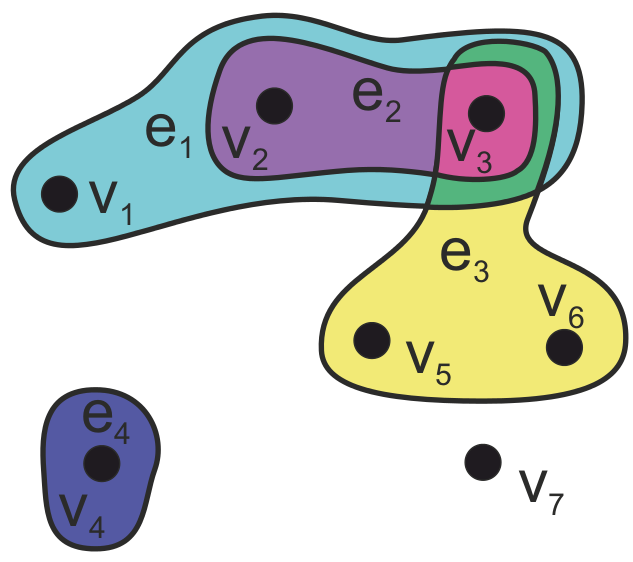
\includegraphics[width=0.6\textwidth, angle=0]{files/Hypergraph.png}
	\caption[Reprezentace hypergrafu]{Reprezentace hypergrafu}\label{fig:hypergraph}
\end{figure}

\medskip
$\prod = {V_1, V_2, ..., V_k} $ je K-way partition grafu H, pokud jsou dodrženy následující podmínky.
\begin{itemize}
\item každý segment $V_k$ je neprázdná podmnožina $V$, tedy $V_k \subseteq V$ a $V_k = 0$ pro $1 \leq k \leq K$
\item segmenty jsou párově disjunktní tedy $V_k \cap V = 0 $ pro všechna $1 \leq k \leq K$
\item sjednocení všech $K$ segmentů se rovná $V$
\end{itemize}

\subsubsection{Rekurzivní bisekce}
Problém k-way partitioning grafů/hypergrafů se obvykle řeší za pomoci rekurzivní bisekce. Princip je znázorněn na obrázku \ref{figbisection}. Proběhne tedy nejdříve rozdělení grafu na dva stejně velké segmenty a pak se stejný postup aplikuje na vzniklé podgrafy. Po $log_2K$ fázích je hypergraf rozdělen na $K$ segmentů. Program PaToh, který bude v práci pro řešení této úlohy používán, však dokáže rozdělit graf pomocí rekurzivní bisekce na libovolných $K$ segmentů. Není tedy při volbě počtu segmentů omezený na používání hodnot jež jsou mocniny dvou. Více o tomto problému je poskytnuto v manuálu\footnote{\texttt{http://bmi.osu.edu/umit/PaToH/manual.pdf}} pro tento nástroj. 




\begin{figure}[h]\centering
	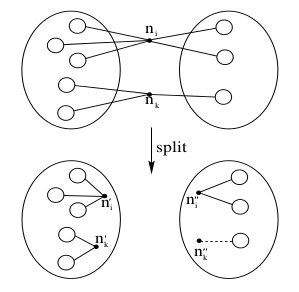
\includegraphics[width=0.6\textwidth, angle=0]{files/bisection.png}
	\caption[bisekce hypergrafu]{bisekce hypergrafu}\label{figbisection}
\end{figure}


\chapter{Existující řešení pro optimalizaci distribuce dat v MapReduce}
V této kapitole bude představeno řešení, které poskytl M. Liroz-Gistau et al. ve svém článku Data Partitioning for Minimizing Transfered Data in MapReduce \cite{gistau}. V tomto článku se zaměřují na redukování datových přenosů mezi mapovací a redukční fází. V tomto místě přichází na řadu fáze, kde probíhá míchání intermediate klíčů(shuffle phase). Od tohoto řešení se bude poté odvíjet návrh řešení pro databázi HBase. Protože v předchozích kapitolách už byl vysvětlen princip zpracování dat pomocí Map Reduce, může tato kapitola plynule navázat na tyto poznatky. 

\section{Definice problému}
Nejdříve je zapotřebí formálně definovat, jaký problém chceme řešit. Mějme tedy sadu MapReduce úloh, které reprezentují typické zatížení systému a sadu vstupních dat. Předpokládejme, že budoucí MapReduce úlohy budou vykonávat podobné úlohy na podobných datech a budou generovat podobné intermediate key (předpokládá se, že v praxi se vykonávají pořád stejné úlohy, jen dochází například ke zvětšování datasetu o nově zapsaná data). 

Cílem navrhovaného systému je automatické rozdělení vstupních dat tak, aby u budoucího vykonávání MapReduce úloh byl minimalizován přenos dat mezi jednotlivými uzly v shuffle fázi. Při tomto rozdělování se nebere v úvahu plánování mapovacích a redukčních fází, ale pouze inteligentní rozdělení intermediate klíčů mezi jednotlivé redukční uzly.

	Definujme daný problém formálně. Mějme vstupní data pro MapReduce úlohu $job_\alpha$ složená z jednotlivých souborů $D = \{d_1, ..., d_n\}$, které jsou rozděleny do  množiny bloků (chunks) $C = \{c_1, ..., c_p\}$. Funkce $loc : D \rightarrow C$ přiřazuje data do bloků. Nechť  $job_\alpha$ je složen z $M_\alpha = \{m_1, ..., m_p\}$ mapovacích úloh a $R_\alpha = \{r_1, ..., r_q\}$ jsou redukční úlohy. Předpokládejme, že každá mapovací úloha $m_i$ zpracuje blok $c_i$. Nechť  $N_\alpha = \{n_1, ..., n_s\}$ je množina výpočetních uzlů použitých pro provedení úlohy. $node(t)$ reprezentuje výpočetní uzel, kde se vykonává úloha $t$.

Nechť $I_\alpha = \{i_1, ..., i_m\}$ je množina intermediate párů klíč-hodnota produkovaných mapovací fází jako je $map(d_j) = \{i_{j_1}, ..., i_{j_t}\}$. $k(i_j)$ reprezentuje klíč z intermediate páru $i_j$ a $size(i_j)$ reprezentuje celkovou velikost v bytech. Definujeme $output(m_i) \subseteq I_\alpha$ jako množinu intermediate párů produkovaných mapovací úlohou $m_i$, tedy $output(m_i) = \bigcup_{{d_j}\in{c_i}} map(d_j)$. Dále definujeme $input(r_i)\subseteq I_\alpha$ jako množinu intermediate párů přiřazených k redukční úloze $r_i$. Funkce $part : k(I_\alpha) \rightarrow R$ přiřazuje intermediate klíč k redukční úloze. 

Nechť $i_j$ je intermediate klíč-hodnota pár, pak  $i_j \in output(m)$ a $i_j \in input(r)$. Nechť $P_{i_j} \in {0,1}$ je proměnná, která se rovná 0 pokud intermediate pár $i_j$ je vyprodukován na stejném výpočetním uzlu jako je následně zpracováván v redukční části a 1 v opačném případě.  

Nechť $W = {job_1, ..., job_w}$ je množina všech úloh. Cílem je pak najít optimální $loc$ a $part$ funkce tak aby $\sum_{job_\alpha \in W} \sum_{i_j \in I_\alpha}  size(i_j)P(i_j) $ bylo minimální.

\section{MR-part}
Pro vyřešení zadaného problému byla navržena technika pojmenovaná MR-Part. Tato technika, za pomocí automatického dělení vstupních souborů, dovoluje využití maximální výhody data-locality při plánování redukčních úloh a výrazně snižuje množství dat, které je potřeba přesunout v shuffle fázi. MR-part se skládá ze tří hlavních fází. Jedná se o fáze Workload Monitoring, Partitioning a Execution and scheduling, tak jak je vidět z obrázku \ref{fig:MR-part}. V první fázi se shromáždují informace o vykonávání jednotlivých MapReduce úloh, které jsou následně zkombinovány. Z těchto informací je vytvořen model zatížení pomocí hypergrafu. V druhé fázi se na vytvořený hypergraf aplikuje dělící algoritmus, který rozdělí data na požadovaný počet bloků a následně jsou vstupní soubory upraveny na základě tohoto rozdělení. V poslední fázi se využije upravených vstupních souborů a za pomoci optimalizace přiřazování redukčních úloh se dosáhne minimalizace přenosu dat v shuffle fázi.

\begin{figure}\centering
	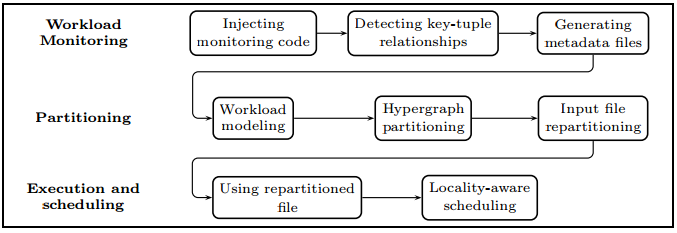
\includegraphics[width=1\textwidth, angle=0]{files/MR-part}
	\caption[MR-part schéma]{MR-part schéma}\label{fig:MR-part}
\end{figure}

\subsection{První fáze - Workload Characterization}
Pro zajištění minimalizace přenosů mezi výpočetními uzly při přechodu z mapovací do redukční fáze je nejdříve zapotřebí zjistit, jaké páry hodnot se generují pro vstupní data a následně je vhodně seskupit. K tomu dochází v monitorovací a kombinační části první fáze.
\paragraph{Monitoring}
Nejprve je zapotřebí získat potřebná data z typických MapReduce úloh, u kterých se očekává jejich častější vykonávání. K zachycení těchto dat se využívá třída  \texttt{RecordReader} \footnote{\texttt{RecordReader} je třída, která parsuje vstupní soubor a generuje vstupní páry. Každý datový formát má jiný \texttt{RecordReader}. Soubory tedy obvykle používají stále stejný.} , která je rozšířená o  monitorovací funkci. Monitorovací funkce unikátně identifikuje vstupní páry klíč-hodnota a jejich pozici ve vstupních datech. Pro každou mapovací úlohu se tak vytvoří soubor s metadaty. Vždy, když je načten nový blok s daty, je zároveň vytvořen i nový soubor obsahující informace o bloku. Následně je iniciován record counter($rc$). Pokaždé, když je načten vstupní pár, inkrementuje se counter o 1. Poté pokud dojde k vytvoření vstupního páru, je vygenerován pár $(k, rc)$. Po dokončení zpracování bloku dat jsou takto vygenerované páry uloženy do již vytvořeného souboru ve formátu $\langle k,\{rc_1, ..., rc_n\}\rangle$ tedy klíč a za ním následně identifikátory řádku, které tento klíč generují.
\paragraph{Combination}
Následující fáze již neběží zároveň s jinými úlohami, ale pustí je uživatel ideálně v čase, kdy systém není vytížen jinými výpočty. V kombinační fázi se shromáždí a zkombinují metadata z monitorování a na jejich základě se vygeneruje pro každý vstupní soubor hypergraf. Hypergraf $H = (H_V, H_E)$ je graf, kde každá hyperhrana $e \subseteq H_E$ může propojovat více jak dva vrcholy  $v \subseteq H_V$. Po zpracování metadat se pak do tohoto hypergrafu uloží každý zpracovávaný prvek (vygenerovaný unikátní identifikátor reprezentující typicky řádek ve vstupním souboru).  Poté se přidá hyperhrana, reprezentující klíč a propojí vrcholy, které tento klíč vygenerovaly. Detailní popis algoritmu v pseudokódu je zobrazen na obrázku. \ref{fig:alg1}

\begin{figure}\centering
	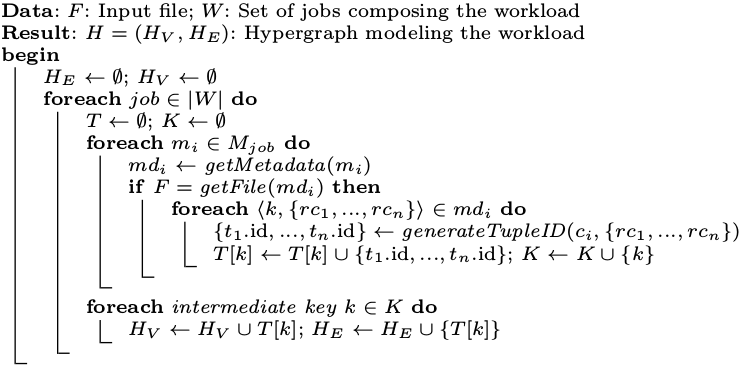
\includegraphics[width=1\textwidth, angle=0]{files/alg1}
	\caption[Pseudokód algoritmu pro Metadata Combination]
	{Pseudokód algoritmu pro Metadata Combination}\label{fig:alg1}
\end{figure} 

\subsection{Druhá fáze - Repartitioning}
Nyní, když je vygenerován hypergraf modelující rozložení dat v jednotlivých souborech, je na každý hypergraf aplikován min-cut k-way dělící algoritmus. Tento algoritmus má jako vstup hodnotu $k$ a hypergraf, ze kterého následně vygeneruje $k$ disjunktních podmožin vrcholů tak, aby byla minimalizována suma hran mezi uzly rozdílných podmnožin. Parametr $k$ je nastaven podle počtu bloků ve vstupním souboru. Po provedení tohoto algoritmu by měly být v jednotlivých vygenerovaných podmnožinách seskupeny uzly generující stejný klíč. Následně se použijí tyto podmnožiny k vygenerování nových vstupních souborů, kde už jsou data seřazena tak, aby řádky generující stejný klíč byly maximálně seskupeny. Tímto nově vzniklým souborem je následně nahrazen starý vstupní soubor, který je smazán. Pseudokód algoritmu je uveden na obrázku. \ref{fig:alg2} V algoritmu je uvedená funkce $RR$, která reprezentuje funkci třídy $RecordReader$  použitou pro parsování vstupních souborů. Dále se v kódu oběvuje funkce $RW$ znamenající $RecordWriter$. Její funkce je inverzní k funkci $RecordReader$. V této části je výpočetně nejsložitější vykonání min-cut algoritmu. Min-cut algoritmus spadá do skupiny NP-Complete problémů. Existuje však několik aproximačních algoritmů, které byly navrženy k řešení tohoto problému. V tomto případě byl použit nástroj \texttt{PaToH} \footnote{\texttt{http://bmi.osu.edu/$\sim$:umit/software.html}}

\begin{figure}\centering
	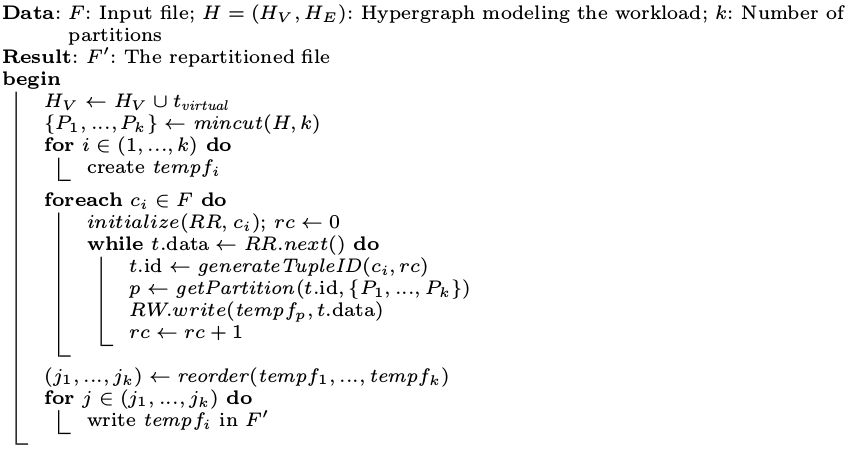
\includegraphics[width=1\textwidth, angle=0]{files/alg2}
	\caption[Pseudokód algoritmu pro Repartitioning]
	{Pseudokód algoritmu pro Repartitioning}\label{fig:alg2}
\end{figure} 

\subsection{Třetí fáze - Execution and scheduling}
K tomu, aby bylo možné plně využít výhody získané přeskupením záznamů v předchozích fázích, je zapotřebí maximalizovat data locality při plánování redukčních úloh. K tomuto účelu byl upraven algoritmus fairness-locality poskytnutý v článku "Locality/fairness-aware key partitioning for mapreduce in the cloud"\cite{cloudcom}, který pro každý pár key-value vypočítá skóre reprezentující poměr mezi vyvážeností vstupů do redukční fáze a lokací dat. Pro každý klíč jsou pak možné uzly seřazeny podle jejich frekvence výskytu v sestupném pořadí (uzly s vyššími frekvencemi mají lepší data locality). Avšak namísto vybrání uzlu s maximální frekvencí se upřednostní uzel s lepším fairness-locality skore. To má za následek maximální vyvážení vstupů do redukčních fází.

V MapReduce frameworku je tedy nutné provést následující modifikace:

\begin{itemize}
  \item Upravení partitioning funkce tak, aby každému intermediate klíči přiřadila vlastní partition.
  \item Po dokončení mapovací části odeslat do master uzlu seznam s vygenerovanými intermediate klíči a jejich frekvencemi. Tato informace je přiložena k Heartbeat zpávě, která je odesílána po dokončení mapovací úlohy.
  \item Master přiřadí  intermediate klíč k redukční úloze na základě dodaných informací a zajístí tak maximální vyvážení a data-locality v redukční části výpočtu.
\end{itemize} 

\section{Testování a výsledky}
MR-Part byl implementován v Hodoop-1.0.4 a otestován na \texttt{Grid5000} \footnote{https://www.grid5000.fr/mediawiki/index.php/Grid5000:Home}. Jedná se o  rozsáhlou infrastrukturu složenou z rozdílných sítí s několika clustery výpočetních uzlů. Nutno podotknout, že tato infrastruktura není typická pro nasazení Hadoopu a vykonávání MapReduce úloh, především právě  kvůli nesourodosti clusterů v síti, jejich fyzické vzdálenosti a tím i kapacitně omezeném propojení. Částečně i proto bylo zrychlení zprácování tak znatelné. K testování byly využity datasety z \texttt{TPC-H} \footnote{http://www.tpc.org/tpch/}. 
\subsection{Výsledky}

\paragraph{Množství přenesených dat pro různé typy dotazů} \hfill \\
Při spustění několika různých úloh \texttt{TPC-H} \footnote{Implementace použitých dotazů: http://www.cs.duke.edu/starfish/mr-apps.html}.  na původních datasetech bylo v shuffle vázi přeneseno cca. 80\% dat. Po provedení dotazů na již upravených datech pak docházelo k přenosu dat  nižším než 10\% pro všechny provedené dotazy.

\paragraph{Množství přenesených dat v závislosti na velikosti clusteru} \hfill \\
Při provedení vybraného dotazu nad konfiguracemi systému s různým počtem clusterů nedocházelo k žádné výrazné změně v podílu přenesených dat. Jednalo se o konfigurace o pěti až dvacetipěti uzlech v clusteru.

\paragraph{Časová náročnost dotazů} \hfill \\
Jak již bylo řečeno, časová náročnost je velmi vázaná na propustnost sítě. Bylo provedeno vykonání dotazů na různých šířkách pásma a výsledek byl očekávaný. Tedy čím pomalejší síť mezi výpočetními uzly, tím výraznější zrychlení při vykonávání dotazů.






\chapter{Návrh řešení pro HBase}
Při návrhu řešení pro optimalizaci umístění dat na výpočetní uzly minimalizující datové přenosy v databázi HBase jsem vycházel z již navrhnutého a implementovaného řešení pro souborový systém HDFS, které jsem popsal v předchozí kapitole. Nebudu proto uvádět znovu celý návrh řešení, ale začátek této kapitoly pojmu jako výčet nutných změn, oproti návrhu pro implementaci v HDFS. V druhé části se budu věnovat především návrhu cílového rozložení dat na jednotlivé region servery.

\section{Řazení záznamů v databázi}
Jedna ze základních změn při návrhu optimalizace pro databázi HBase oproti návrhu pro HDFS je fyzické uložení jednotlivých řádků, tedy záznamů, v databázi. Nativní funkcí HBase je ukládání záznamů v lexikografickém pořadí. Tato funkce je pro HBase klíčová a je charakteristickým prvkem, kterým se odlišuje od jiných databází. Právě tato vlastnost dává HBase velkou sílu při sekvenčním prohledávání ať už celého datasetu nebo určité "výseče" z dat. Tento fakt se ale přímo rozchází se základní myšlenkou optimalizace pro HDFS, kdy je nezbytné změnit fyzické pořadí a tím i uložení záznamů. 
Je tedy nutné navrhnout optimální řešení, jak docílit toho, aby bylo možné změnit pořadí záznamů v závislosti na požadavcích optimalizačního algoritmu. V úvahu přicházejí dvě možné varianty, jak se s tímto omezením vyrovnat. Prvním z možných řešení je změna klíče dle potřeb optimalizačního algoritmu, druhým řešením je přidání prefixu k již existujícímu klíči tak jak je naznačeno na obrázku \ref{fig:keys}. Pro výběr optimálního přístupu můžeme tyto dvě varianty porovnat:



\begin{description}
\item[Změna klíče řádku podle potřeb optimalizačního algoritmu] \hfill \\
 Toto řešení se nabízí jako nejjednodušší. Naráží však na výrazný problém. Při návrhu logického modelu pro databáze v HBase se typicky jako klíč pro jednotlivé záznamy používá klíč nesoucí určitou informační hodnotu (například část klíče odpovídá času pořízení daného záznamu). Změnu klíčů by jsme si tedy v tomto případě nemohli dovolit. Pro aplikování tohoto přístupu by se nabízely tabulky, kde je klíč automaticky generován a nenese žádnou další informaci mající spojitost s daty nachazéjícími se v řádku, který reprezentuje.
 
 \item[Přidání prefixu k již existujícímu klíči] \hfill \\
 Druhým možným řešením je přidání prefixu k již existujícímu klíči. Tento návrh již řeší problém s automatickým řazením, zároveň přidání krátkého prefixu neznehodnotí informaci uloženou v klíči Jen je nutné při dalších dotazech toto zohlednit a před zpracováním dat prefix z klíče dočasně po dobu zpracování odstranit nebo jinak zohlednit. Nabízí se více možností, na jakém základě prefixy přiřazovat. Nejefektivnější je přidání určité hodnoty v bitech, na základě požadovaného počtu segmentů výsledného rozdělení grafu. 
 
 \begin{figure}[h]\centering
	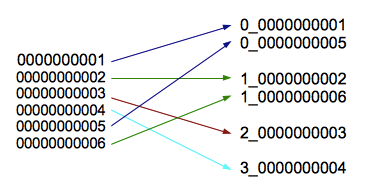
\includegraphics[width=0.8\textwidth, angle=0]{files/rows}
	\caption[Řazení řádků za pomoci přidání prefixu]
	{Řazení řádků za pomoci přidání prefixu}\label{fig:keys}
\end{figure} 
 
\end{description} 

Využijeme tedy pro nás vhodnější přidávání prefixu. Je však nutné při výmýšlení v jakém tvaru prefix ke klíči přidáme, zohlednit i fakt, že se do databáze i nadále budou přidávat nová data. Prefix tedy musí být zvolen tak, aby nově přidávané řádky měly originální klíč takové hodnoty, aby se mohl řádek přidat až za skupinu klíčů s prefixy. Toto je zapotřebí zajistit především ze dvou důvodů:

\begin{itemize}
\item Databáze HBase není navržena a ani určena pro častý náhodný přístup k datům, tím spíše pro vkládání dat na náhodná místa. Tím, že by se nově vzniklé řádky ukládaly díky lexikografickému pořadí napříč celou tabulkou, by docházelo k velké zátěži serveru plynoucí z nutnosti přesouvat velké množství dat tak, aby se řádky mohly vložit na svoje místo.
 
\item Při vkládání řádků na náhodná místa v databázi by se postupně rozbila vzniklá struktura, kdy řádky generující stejný klíč jsou seřazeny a byly by postupně ředěny nově uloženými řádky a tím by klesala následně účinnost datové optimalizace. 
\end{itemize}

Tímto však nastává problém. jak řazení na konec tabulky optimálně dosáhnout. V případě, že by nové klíče měli díky své struktuře vždy klíč lexikograficky zařaditelný až za klíče s prefixem, by se nic řešit nemuselo. V obecném případě se ale nelze na toto spolehnout a je žádoucí nově vzniklé klíče taktéž opatřit prefixem symbolizujícím, že řádky s těmito klíči nebyly zatím zpracovány a zajistit tím tak i to, že se tyto řádky budou ukládat na konec tabulky. V případě, že se nashromáždil velký počet takto nově příchozích záznamů je pak na zvážení spustit optimalizaci znovu. Ve výsledku tedy vytvořit novou tabulku naplněnou řádky s již novými prefixy. 

\subsection{Fyzické uložení family column}
Ačkoli jsou řádky ukládány lexikograficky, v každém stores jsou takto uloženy pouze hodnoty v rámci jedné family. Každá family sloupců se tedy ukládá do oddělených stores. Platí však omezení, že ačkoli jsou jednotlivé families řádků uloženy rozděleně, vždy jsou tyto části uložené v rámci jednoho regionu. Dojde-li tedy k přejmenování identifikátoru řádku, repsektive vytvoření nové tabulky s prefixem, budou řádky o určitém rozsahu klíčů vždy uloženy logicky v jednom HRegionu. Vzhledem k tomu, že optimalizaci budeme provádět pro seskupení řádků v rámci regionu, není zapotřebí tento fakt jakkoli zohledňovat. Při určování rozdělení dat do segmentů se nemusí tedy řešit počet a mohutnost families v tabulkách a je možné na řádek nahlížet jako na celek.


\section{Splitting HBase regionů}
V návrhu pro implementaci v HBase je zapotřebí zohlednit, jak pracovat s distribucí HBase regionů do souborového systému. Jak již bylo řečeno, v HBase se data v řádcích ukládají do HBase regionů, kde je vždy uložen určitý rozsah lexikograficky seřazených řádků. Řádek je vždy uložen jako celek jen na jednom HRegionu. Není tedy potřeba speciálně ošetřovat případné dělení řádku. 

Tabulky se typicky skládají z mnoha regionů, které jsou umístěny na menším počtu region serverů. Regiony tedy slouží jako mechanizmus k rozložení zátěže napříč clusterem. Vždy když se vytváří nová tabulka, vytvoří se pouze jeden region, který se postupně při nabírání objemu štěpí na více regionů, které se distribuují v clusteru. Proto ve fázi nahrávání dat do DB není využita plná kapacita clusteru. Toto chování je zapříčiněno především tím, že dopředu není zřejmé, kde se budou ve výsledné tabulce nalézat split points, tedy místa, kde dojde k rozdělení tabulky na více regionů. Tyto body jsou totiž špatně predikovatelné, zejména kvůli faktu že rozložení klíčů v tabulce nemusí být vždy rovnoměrné. V našem případě však již víme, s jakým rozložením dat budeme pracovat při vytváření tabulky a zároveň budeme vědět, na kolik částí budeme chtít data rozdělit. Ideální stav by tedy byl, že výsledná skupina řádků určená dělícím algoritmem jako homogenní segment by byla uložena na určitém počtu regionů aniž by v těchto regionech byla uložena data z ostatních částí tabulky. K tomuto rozdělení, můžeme využít pre-splitting \cite{split}.

\subsection{Pre-Splitting}
Pre-splitting je nástroj, který nám umožňuje vytvořit novou tabulku s již vytvořenými split pointy. Použití tohoto nástroje nám umožní vytvořit si tabulku podle našich potřeb. První z možných řešení je předpočítání splitting pointů podle zadaných kritérií. K tomu slouží \texttt{regionSplitter} utility. RegionSplitter vytvoří splitting points pomocí \texttt{SplitAlgorithm}. Předdefinováné algoritmy jsou \texttt{HexStringSplit} a \texttt{UniformSplit}. První algoritmus je možné použít, pokud klíče obsahují prefixy ve formě hexadecimálního řetězce. Druhý algoritmus určuje splitting point pomocí uniformního rozdělení klíčů. Pro potřeby naší aplikace se nabízí využití prvního algoritmu, kdy dojde k rozdělení podle prefixů, které byli ke klíčům přidány na základě výsledku dělícího algoritmu. Je možné implementovat i vlastní \texttt{SplitAlgorithm}, nicméně pro naše potřeby je plně dostačující již implementovaný algoritmus.

Následující příkaz vytvoří tabulku testTable, kde -c 10 definuje počet regionů a -f f1 definuje požadované families v tabulce.

\medskip
\begin{lstlisting}[frame=single]  % Start your code-block
ds
$ hbase org.apache.hadoop.hbase.util.RegionSplitter \
> testTable HexStringSplit -c 10 -f f1

\end{lstlisting}
\medskip
Následně dojde k vygenerování tabulky o deseti regionech. Výpis udává i konkrétní \texttt{STARTKEY} a \texttt{ENDKEY} pro každý region. 
\medskip
\begin{lstlisting}[frame=single]  % Start your code-block
 
15/04/08 18:49:32 DEBUG hbase.HRegionInfo:
> Current INFO from scan results = 
> {NAME =&gt;> 'test_table,,
> 135856377.acc1ad1b7962564fc3a43e5907e8db33.', 
> STARTKEY =&gt; '', ENDKEY =&gt; '19999999', 
> ENCODED =&gt; acc1ad1b7962564fc3a43e5907e8db33,}
15/04/08 18:49:32 DEBUG hbase.HRegionInfo: 
> Current INFO from scan results = 
> {NAME =&gt; 'test_table,
> 19999999,135856377.37ec12df6bd0078f5573565af415c91b.', 
> STARTKEY =&gt; '19999999', ENDKEY =&gt; '33333332', 
> ENCODED =&gt; 37ec12df6bd0078f5573565af415c91b,}
...

\end{lstlisting}
\pagebreak
\subsection{Auto Splitting}
Jak již bylo řečeno, pre-splitting je nástroj, který má na starosti rozdělení tabulky při jejím vytvoření v případě, že nechceme začít vkládat do defaultní tabulky s jedním regionem. Nehledě na to, zda pre-splitting použijeme nebo ne, je potřeba nadále spravovat regiony v závisloti na nově přidávaných datech. K tomu slouží Auto splitting, který automaticky rozděluje regiony, které dosáhly své maximální velikosti. Nastavení automatického dělení regionů je možné provést pomocí \texttt{RegionSplitPolicy} API. K dispozici jsou tři předdefinované varianty:

\begin{itemize}
	\item ConstantSizeRegionSplitPolicy
	\item IncreasingToUpperBoundRegionSplitPolicy
	\item KeyPrefixRegionSplitPolicy
\end{itemize} 

\subsubsection{ConstantSizeRegionSplitPolicy}
Jedná se o jednoduchou politiku (ve starších verzích před verzí 0.94 to byla defaultní a jediná předdefinovaná) k určení, kdy má dojít k rozdělení regionu. Rozdělení nastane v případě, kdy dojde k překročení maximální velikosti alespoň jednoho store file v regionu (uložiště jedné family v rámci regionu). Tato hodnota je konfigurována v \texttt{hbase.hregion.max.filesize} a její defaultní hodnota je 10 GB. 

\subsubsection{IncreasingToUpperBoundRegionSplitPolicy}
Pro novější verze je defaultní \texttt{IncreasingToUpperBoundRegionSplitPolicy}. Tato politika provádí více agresivní splitting  založený na počtu regionů uložených v region serverech. K určení velikosti při které dojde k rozdělení regionu se používá vzorec \\  $MIN(R^2 * hbase.hregion.memstore.flush.size,hbase.hregion.max.filesize)$. \\ kde $R$ je počet regionů stejné tabulky na jednom regionserveru. Například uvažujme situaci, kdy máme nastavenou default memstore flush size na defaultní hodnotu 128MB a hodnotu max store size na defaultních 10GB. K prvnímu splitu dojde po provedení první operace flush, při velikosti 128MB. Postupně, jak bude docházet ke zvyšování počtu regionů v region serveru, bude zároveň docházet i ke zvětšování velikosti jednotlivých regionů a to konkrétně na 512MB, 1152MB, 2GB, 3.2GB, 4.6GB, 6.2GB, etc. Po dosažení 9 regionů se zvětšování zastaví díky \texttt{hbase.hregion.max.filesize} nastavené na 10 GB. U obou předchozích metod dochází při dělení vždy k rozdělení v místě, kde je prostřední bod největšího store file.


\subsubsection{KeyPrefixRegionSplitPolicy}
Poslední z předdefinovaných politik pro automatický splitting je politika \\ \texttt{KeyPrefixRegionSplitPolicy}. V tomto případě se rozdělení provádí za pomocí prefixu. Na základě určení velikosti prefixu dojde k jejich rozdělení do skupin. Tato funkce pak zajistí, že při dělení regionů nedojde k rozdělení uprostřed takto definované skupiny. Dojde tedy k situaci, kdy jsou klíče se stejným prefixem uloženy v rámci jednoho regionu (nebo více regionů v případě, že velikost těchto dat překročí maximální povolenou velikost regionu).

\subsection{Určení optimální politiky}
Při porovnání těchto předem definovaných politik jsem došel k závěru, že politika \texttt{KeyPrefixRegionSplitPolicy} přesně splňuje požadavky plynoucí z potřeby ukládat předem definované rozsahy řádku pomocí prefixu v rámci jednoho regionu. Je zde také možnost naimplemetovat vlastní politiky, nicméně v tomto případě plně vyhovuje již definovaná politika. Vzhledem k tomu, že řádky v tabulkách nemají z pravidla stejnou délku, nelze dělení regionů řešit příliš přesným způsobem, například určit přímo velikost regionu. Tato politika zaručí volnost při rozdělování regionů a zajistí seskupení požadovaných dat do jednoho či více regionů, nehledě na maximální velikost regionu.

\section{Provedení partitioningu}
V této fázi, kdy je již zajištěno správné rozdělení a nastavení nové tabulky, se může přejít k samotnému repartitioningu. Je nutné zpracovat vygenerované metadata s informacemi o uzlech a vytvořit z nich strukturu hypergrafu. Samotný výpočet rozdělení hypergrafu se provede za pomoci externího programu, proto se musí vygenerovat i vstupní data pro tento program. Nakonec se data vygenerovaná PaToH programem zpracují a podle nich se jednotlivé segmenty postupně zapíší do nové databáze. Na konci dojde ke smazání původní databáze a přejmenování nové na původní.
\subsection{program PaToH}
Při kombinační části je zapotřebí rozdělit co nejoptimálněji vzniklý hypergraf. Tato fáze je klíčová a právě správné rozdělení grafu je klíčem k následnému optimálnímu rozložení dat. K vyřešení této úlohy použiji již naimplementovaný nástroj pro dělení hypergrafů PaToH\footnote{http://bmi.osu.edu/ \textasciitilde umit/software.html}. Program nabízí 2 možnosti použití. Buď jako stand-alone program spustitelný z příkazové řádky nebo jako knihovna v jazyku C. Vzhledem k tomu, že pro naše potřeby plně dostačuje rozhraní spustitelného programu, využiji této možnosti a v implementaci provedu výpočet spuštěním příkazu z kódu. Použití knihovny by nejspíše urychlilo výpočet, především při zajištění optimálního nastavení algoritmu pro výpočet. Detailní optimalizace algoritmu pro partitioning hypergrafů však není předmětem této práce a tak využijeme pouze základní funkčnost, která vede i tak k plně dostačujícím výsledkům.

\subsection{Použití programu}
Program je možné spustit z příkazové řádky pomocí příkazu ve tvaru:
\medskip
\begin{lstlisting}[frame=single]  % Start your code-block
 
> patoh <hgraph-file> <num-of-parts> [[par1] [par2] ....]

\end{lstlisting}
\medskip

První dva argumenty jsou povinné a určují vstupní soubor obsahující reprezentaci hypergrafu a počet části požadovaného rozdělení. Následující paramery jsou volitelné a určují nepovinné nastavení výpočetního algoritmu.  Tyto parametry se zadávají pomocí dvoupísmenné zkratky následované rovnítkem a zadanou hodnotou. V našem případě použijeme defaultní nastavení. Pokud by bylo zapotřebí výpočet rozdělení grafu optimalizovat, je možné toho docílit právě přidáním patřičních parametrů pro výpočet. Přehled volitelných parametrů je uveden v manuálu k tomuto programu. Po spuštění a proběhnutí programu se vytvoří výstupní soubor a v konzoli se zobrazí takto formátovaná statistika výpočtu značící úspěšné rozdělení hypergrafu:
\medskip
\begin{lstlisting}[frame=single]  % Start your code-block
 
> patoh ken-11.u 4 RA=6 UM=U 
 
 
+++++++++++++++++++++++++++++++++++++++++++++++++++++++
+++ PaToH v3.2 (c) Nov 1999-, by Umit V. Catalyurek
+++ Build Date: Sun Mar 13 17:41:19 2011 -0400
+++++++++++++++++++++++++++++++++++++++++++++++++++++++
*******************************************************
Hypergraph:ken-11.u #Cells:14694 #Nets:14694 #Pins:82454
*******************************************************
4-way partitioning results of PaToH:
Cut Cost: 4775
Part Weights : Min= 20408 (0.010) Max= 20947 (0.016)
-------------------------------------------------------
I/O : 0.007 sec
I.Perm/Cons.H: 0.002 sec ( 0.7%)
Coarsening : 0.087 sec (37.9%)
Partitioning : 0.011 sec ( 4.8%)
Uncoarsening : 0.128 sec (55.8%)
Total : 0.229 sec
Total (w I/O): 0.236 sec
-------------------------------------------------------

\end{lstlisting}
\medskip
\subsubsection{Vstupní formát dat}
Vstupní hypergraf je reprezentován textovým souborem. První řádek souboru obsahuje informace o celém grafu. Následující řádky pak obsahují informace o každé hyperhraně v grafu. První řádek obsahuje 4 až 6 hodnot. Hodnoty postupně udávají:
\begin{itemize}
\item index base (O nebo 1) značíci od jakého čísla indexujeme elementy v grafu
\item počet uzlů v grafu
\item počet hyperhran v grafu
\item počet pinů (propojení hrany a vrcholu)
\item schéma vážení grafu (volitelné)
\item počet vah pro uzel (volitelné)
\end{itemize}

Následující řádky reprezentují vždy po jedné hyperhraně a udávají indexy uzlů, které hyperhrana propojuje. Možné podoby vstupních souborů jsou ukázány na obrázku \ref{fig:input}

\begin{figure}[h]\centering
	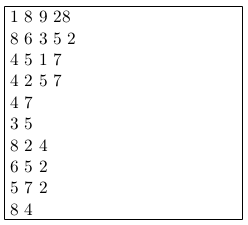
\includegraphics[width=0.4\textwidth, angle=0]{files/inputformat}
	\caption[Vstupní formát hypergrafu]
	{Vstupní formát hypergrafu}\label{fig:input}
\end{figure} 
\subsubsection{Výstupní formát dat}
Po vykonání výpočtu na hypergrafu reprezentovaném souborem input.hygr pomocí PaToH programu, je výsledek uložen v souboru input.hygr.part.K. Kde K značí počet vygenerovaných podgrafů. Tento soubor obsahuje |V| čísel v rozsahu [0, K - 1]. Každé i-té číslo ukazuje do jakého hypergrafu patří i-tý vrchol z původního grafu.



\section{Uložení DB v upravené podobě}
Po provedení  partitioningu je zapotřebí nově vzniklá data zapsat do databáze. Jsou možné dvě řešení. Buď data s nově vzniklými klíči přidat do již existující tabulky a původní záznamy smazat nebo je vložit do tabulky nové a starou smazat poté. Obě možnosti by byli přípustné, ale první návrh by vyžadoval složitější řešení při mazání starých řádků a následném přepočítávání a přerozdělování nových řádků, které v tabulce zůstali, do patřičných regionů. 

Proto při ukládání dat dojde k vytvoření "duplicitní" tabulky do které se nahrají data s novými klíči. Po nahrání dat dojde ke smazání staré databáze a přejmenování nové tabulky podle jména původní. Tím se docílí toho, že nově vzniklá tabulka bude identická s původní. Tedy až na rozdíl v klíčích řádků obohacených o prefix a především tedy vnitřním uložením dat, které však při běžném používání databáze zůstává pro uživatele skryté. 

\section{Určení optimálního počtu segmentů pro dělící algoritmus}
Počet regionů, do kterých se budou nově vytvořená data ukládat je také úkol, u kterého se nabízí odvodit od původního řešení pro HDFS. V původním řešení se určuje počet segmentů, na které se data rozdělí podle počtu vstupních bloků dat. V případě HBase se nabízí využít jako hodnotu pro zvolení počtu segmentů počet HFile souborů, ve kterých je databáze uložena. Nicméně právě zde se tato analogie využít nedá a to především, kvůli tomu, že HBase nenabízí žádné nástroje pro práci s jednotlivými HFile a ty se tak vytváří automaticky v rámci regionu. I v případě, že by bylo možné zapisovat do konkrétních HFile souborů, nebylo by možné tyto soubory nijak efektivně namapovat na vznikající data bloky v HDFS. To není možné z jednoduchého důvodu a to, protože HBase pracuje s HDFS jen jako s datovým uložištěm a nemá žádné nástroje k tomu, aby ovlivňovala samotné uložení dat v HDFS a mohla řídit upravování struktury databloků. Vníma ho pouze jako souvislý úložný prostor. Stejně tak HDFS vnímá soubory, které přicházejí z HBase pouze jako binární soubory bez jakékoli struktury.

Možné řešení je odvodit počet segmentů od počtu regionů. Při tomto řešení bude sice daleko menší granuralita vzniklých datových segmentů, nicméně to nemusí nutně znamenat horší výsledky. Typicky se tabulky rozkládají na desítkách až stovkách regionů, což by mohlo být pro rozdělení dat na smysluplné skupiny postačovat. Samozřejmě se efektivita tohoto řešení bude odvíjet, jak od samotného počtu regionů, tak od složitosti prováděných dotazů a počtu reducerů při jejich vyhodnocování. Rozdělením dat podle počtu regionů se navíc docílí toho, že nakonec v jednotlivých HFilech budou i tak shromážděny záznamy generující podobné klíče, ikdyž s menší přesností, vzhledem k tomu, že takto shromážděné záznamy se nachází ve všech Hfilech v rámci jednoho regionu.

Protože HDFS ukládá soubory vždy v několika replikách, které využívá rovnoměrně, není žádná možnost jak predikovat, která kopie souboru reprezentující část regionu se zrovna použije. HDFS v zájmu zvýšení spolehlivosti ukládá jednotlivé kopie na různé disky a tak je prakticky nemožné zajistit, aby se používaly k výpočtu data ze souborů uložených u sebe. Volba souboru který se použije je tedy kompletně v režii HDFS. Optimalizace se tak prakticky omezuje pouze na to, že v jednotlivých souborech, které se budou postupně načítat ke zpracování, budou data, která generují stejné klíče. Díky tomu nelze aplikovat ani upravit plánování redukčních úloh pomocí fairness-locality algoritmu tak, jak bylo provedeno v řešení pro HDFS. 


Efektivita takového řešení je tedy diskutabilní, pravděpodobně dojde k určité úspoře při přenosech dat. Nicméně jak moc efektivní použítí optimalizace bude a zda se vůbec vyplatí tuto optimalizaci provádět, bude k posouzení až po naimplementování řešení a provedení testovacích výpočtů. Obecně se ale už z návrhu řešení počítá s menší efektivitou než u řešení pro HDFS. 





\chapter{Implementace řešení}
V této kapitole bude představena implementace navrženého řešení. Při popisu implementace budu postupně probírat všechny klíčové partie. Implementace byla provedena v jazyku Java. V javě je napsán celý balík Hadoop a tak se toto řešení nabízí jako nejvhodnější. Pouze pro provedení partitioning algoritmu byl využit již existující program naimplementovaný v jazyku C. 

\section{Monitoring}
V prvním kroce je nutné získat potřebná data, podle kterých se následná optimalizace bude provádět. Je potřeba shromáždit informace o tom, který řádek tabulky generuje jaký klíč nebo jakou množinu klíčů. Sběr těchto dat se realizuje v průběhu vykonávání sady MapReduce úloh, pro které se bude následně celý dataset optimalizovat. K tomu, abychom mohli nasbírat potřebná data je nutné rozšířit HBase třídy \texttt{RecordReader} třídou \texttt{MyRecordReader} a \texttt{TableInputFormatBase}\ref{fig:record} třídou \texttt{MyTableInputFormatBase}\ref{fig:input}. Bylo nutné upravit a přepsat následující metody:

\begin{figure}\centering
	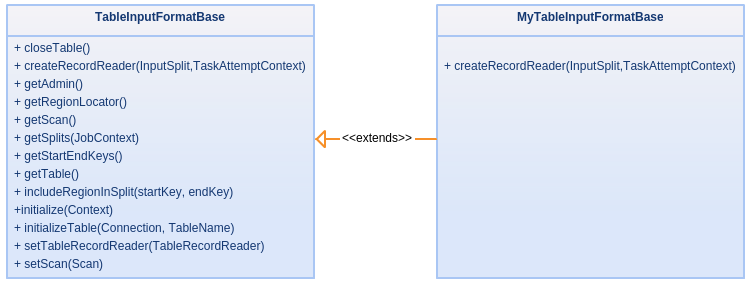
\includegraphics[width=1\textwidth, angle=0]{files/input}
	\caption[Rozšíření třídy TableInputFormatBase]
	{Rozšíření třídy TableInputFormatBase}\label{fig:input}
\end{figure} 

\begin{figure}\centering
	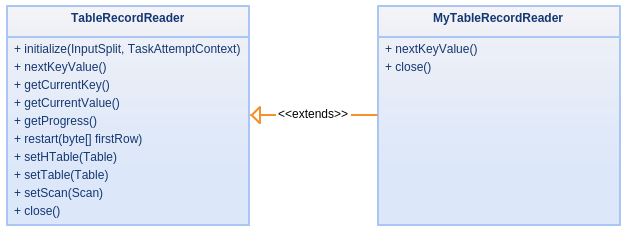
\includegraphics[width=1\textwidth, angle=0]{files/record}
	\caption[Rozšíření třídy RecorReader]
	{Rozšíření třídy RecorReader}\label{fig:record}
\end{figure} 

\begin{description}
\item[TableInputFormatBase] \hfill \\
Nejdříve ověří vstupní konfiguraci pro MapReduce úlohu. Následně \linebreak vytvoří instanci třídy \texttt{RecordReader}, která bude použita k vytvoření key/value párů z načtených dat. Tyto páry jsou pak po jednom zaslány k mapování.

\item[TableRecordReader] \hfill \\
TableRecorReader generuje z dat získaných od \texttt{TableInputFormatBase} key/value páry. Podle zadaného rozsahu projde požadovanou část datasetu, nebo celou tabulku. 
\end{description}

\subsection{MyTableImputClassBase Class}
V této třídě je pouze nutné změnit metodu \texttt{CreateRecordReader} tak, aby \linebreak namísto defaultní TableRecordReader instance nastavila pro prováděnou úlohu instanci record readeru ze třídy \texttt{MyTableRecorReader}.


\subsection{MyTableRecordReader Class}
V této třídě je nutné vytvořit soubor, který uchová vygenerované páry \linebreak key/value, během zpracovávání MapReduce. Při zpracovávání každého \linebreak záznamu se vyhodnotí, zda byl vygenerován klíč. v případě že ano, uloží se do dočasné struktury daný klíč a identifikátor řádku, který ho vygeneroval. Při ukončování úlohy se poté zapíšou získané hodnoty do nově vytvořeného souboru ve formátu:
 $Key;počet\_řádků\_gener.\_klíč;id\_řadku_1 ... id\_řadku_n$. Výsledkem je tedy seznam vygenerovaných klíčů s řádky které tento klíč generují. Instance RecordReaderu se vytváří pro každý zpracovávaný region. Po provedení dotazu tak je vygenerován počet souborů odpovídající počtu regionů na kterých leží zpracovávaná tabulka.


\section{Repartitioning}
Poté co jsme shromáždili potřebná metadata shromažděná při vykonávání MapReduce úloh, je čas přejít k fázi optimalizace rozložení dat. Nyní máme k dispozici soubor nebo několik souborů, kde jsou definovány jednoltivé řádky databáze a k nim seznam klíčů, které generují. Za pomoci dat z těchto souborů je zapotřebí vytvořit strukturu hypergrafu, na který pak následně použijeme partitioning algoritmus.

\subsection{Vytvoření a reprezentace hypergrafu}
Pro reprezentaci hypergrafu jsem použil knihovnu \texttt{Jung}\footnote{\texttt{http://jung.sourceforge.net/}} poskytující implementace různých typů grafů mezi nimiž je i námi požadovaný hypargraf. Při parsování vstupních souborů se postupně vytváří hypergraf.  Každý řádek reprezentuje hyperhranu a vrcholy které jsou touto hranou propojeny. Vždy se tedy vytvoří nová hyperhrana, nesoucí jako svůj identifikátor jméno generovaného klíče, který reprezentuje a postupně ověřuje existenci uzlů, které by měla propojovat. V případě, že uzel neexistuje, vytvoří ho a přidá jako jeden ze svých vrcholů. V opačném případě si pouze přidá již existující uzel. Po dokončení parsování souborů s metadaty tedy máme k dispozici strukturu $setHypergraph$ reprezentující kompletní rozložení zátěže datasetu při vykonávání zadaných dotazů.

\subsection{příprava dat pro Min-cut algoritmus}
Provedení partitioningu na vzniklém hypergrafu má na starosti třída \texttt{MinCut}. Samotné rozdělení grafu pomocí min-cut algoritmus je prováděno za pomoci externího programu PaToH. Nicméně tento program požaduje specifický formát vstupního souboru. Tento soubor je tedy zapotřebí vygenerovat ze stávající reprezentace grafu, jak již bylo popsáno v dřívější kapitole. PaToH očekává jako vstupní soubor graf v podobě od 0 nebo 1 indexovaný seznam hran a vrcholů jež propojuje.  Vytvořil jsem tedy dvě pole $nodesArray$ a $edgesArray$, do kterých se postupně uloží všechny vrcholy a hrany. K vytvoření polí slouží metody \texttt{mapNodes()} a \texttt{mapEdges()}. Zde je uvedena metoda \texttt{mapNodes()}, metoda \texttt{mapEdges()} je analogická.

\begin{lstlisting}[frame=single]  % Start your code-block
    
    private static void mapNodes() {
        nodes = 0;
        Collection<String> S = hypergraph.getVertices();

        for (String key : S) {
            nodesArray.add(nodes++, key);
        }
    }
\end{lstlisting}

Indexy těchto polí pak slouží k vygenerování požadovaného formátu pro PaToH program. Do vytvářeného souboru nejprve uložím hlavičku souboru ve tvaru 0 znamenající výchozí hodnotu indexování a následně počet vrcholů, hran a pinů v grafu. Tyto hodnoty lze jednoduše získat z reprezentace hypergrafu pomocí metod $getVertices()$, $getEdges()$ a počet pinů pomocí metody pro každý uzel $degree(node)$ a sečtené přes všechny uzly v grafu.
Dále je nutné nastavit, na kolik segmentů se má hypergraf rozdělit. Počet segmentů určíme podle počtu regionů v původní tabulce. K tomu slouží metoda \texttt{getNumberOfRegions} ve třídě \texttt{Repartitioning}.
\begin{lstlisting}[frame=single]  % Start your code-block

public int getNumberOfRegions(HTable table){
        List<HRegionInfo> listOfRegion = hbase.getTableRegions(table.getTableName());
        return listOfRegion.size();
    }


\end{lstlisting}
\subsection{Spuštění PaToH a zpracování výsledků}
Nyní již může dojít k zavolání PaToH programu:
\begin{lstlisting}[frame=single]  % Start your code-block

String command = "/patoh ./patohGraph.txt 4 RA=6 UM=U";
Process p = Runtime.getRuntime().exec(command);
\end{lstlisting}

Po dokončení běhu programu máme vygenerovaný soubor, ve kterém je uložena řada čísel reprezentující všechny uzly hypergrafu v pořadí v jakém byli ve vstupním souboru. Hodnota čísla pak určuje do kterého segmentu bude uzel spadat. Pokud tedy například dělíme hypergraf na 4 segmenty, bude v souboru řada čísel o hodnotách 0, 1, 2 a 3. 

Nyní je zapotřebí tyto informace zkombinovat s původním hypergrafem. Třída \texttt{MinCut} vytvoří mapu \texttt{partitionedGraph} a vyplní ji postupně tak, že klíč v mapě je originální klíč z grafu načtený kvůli dodržení pořadí z pole \texttt{nodesArray} a jako hodnota je uloženo číslo segmentu, do kterého daný uzel bude spadat načtené ze souboru vygenerovaného programem PaToH. Výstupem  pak je právě tato mapa, podle které se může provést rozmístění řádků z původní tabulky do nově vzniklé.

\subsection{Vytvoření a konfigurace nové tabulky}
Dalším krokem je vytvoření nové databáze, kterou nahradíme databázi původní. Nejdříve je nutné získat seznam families z původní tabulky. Protože families se na rozdíl o d sloupců musí přidat při vytváření tabulky. Families z původni tabulky získáme následovně. \pagebreak


\begin{lstlisting}[frame=single]  % Start your code-block

originalTable = new HTable(conf, originalDB);
HTableDescriptor originalDBdescriptor = new HTableDescriptor(originalTable);
Set families = originalDBdescriptor.getFamiliesKeys();
\end{lstlisting}
Získané bitové identifikátory jednotlivých family následně využijeme k vytvoření nové instance třídy \texttt{HTableDescriptor}, která reprezentuje tabulku v HBase a nastavíme jí totožné families.
\begin{lstlisting}[frame=single]  % Start your code-block
HTableDescriptor newDBdesctiptor = new HTableDescriptor(newDB);

for (Object family : families) {
    HColumnDescriptor newFamily = new HColumnDescriptor((byte[])family);
    newDBdesctiptor.addFamily(newFamily);
        }
\end{lstlisting}
Ješte před zapsáním nové tabulky na disk musíme nastavit \texttt{Split policy}  na \texttt{KeyPrefixRegionSplitPolicy}, jak jsme se rozhodli při návrhu řešení a nastavíme velikost prefixu, podle kterého se budou v budoucí tabulce záznamy řadit.
\begin{lstlisting}[frame=single]  % Start your code-block

newDBdesctiptor.setValue(HTableDescriptor.SPLIT_POLICY, KeyPrefixRegionSplitPolicy.class.getName());
newDBdesctiptor.setValue(KeyPrefixRegionSplitPolicy.PREFIX_LENGTH_KEY, 
Integer.toString(regions)     );
\end{lstlisting}

Tímto nastavením docílíme toho, že se nová tabulka vytvoří podle tabulky původní a seskupené řádky se uloží podle prefixu přesně podle požadovaného rozdělení.
\subsection{přesun upravených dat}
Po vytvoření nové tabulky přichází na řadu transfer dat z původní tabulky a opatření původních klíčů prefixem podle určeného cílového regionu. Toho docílíme postupným procházením mapy, kde máme seřazeny řádky a k nim přiřazeny cílové regiony. Pro každý záznam se podle klíče najde daný řádek v původní tabulce. Klíč se následně opatří prefixem a vytvoří se v nové tabulce řádek s tímto upraveným klíčem. Poté se načtou hodnoty ze všech sloupců z původní tabulky a tyto data se pak uloží do nové tabulky. Po dokončení tohoto kroku jsou tedy v databázi jak původní tak nová optimalizovaná tabulka. V případě, že situace nenabízí využití takového množství volného místa v databází, je možné databázi vytvářet postupně a již přesunuté řádky postupně mazat. 
\subsection{Smazání původní a přejmenování nové tabulky}
Nakonec je ještě zapotřebí smazat původní tabulku a nově vzniklou tabulku pojmenovat po původní tak, aby jí nahradila. Smazání tabulky lze provést jednoduše.
\begin{lstlisting}[frame=single]  % Start your code-block

void delete(Admin admin, String oldTableName) {
  admin.disableTable(oldTableName);
  admin.deleteTable(oldTableName);
}
\end{lstlisting}
 Přejmenování tabulky ale není možné provést v HBase přímo\cite{HBaseWEB} a tak je nutné nejdříve vytvořit snapshot původní tabulky a z tohoto snapshotu naklonovat novou tabulku s požadovaným jménem. Poté se může snapshot a původní tabulka smazat.

\begin{lstlisting}[frame=single]  % Start your code-block

void rename(Admin admin, String oldTableName, String newTableName) {
  String snapshotName = randomName();
  admin.disableTable(oldTableName);
  admin.snapshot(snapshotName, oldTableName);
  admin.cloneSnapshot(snapshotName, newTableName);
  admin.deleteSnapshot(snapshotName);
  admin.deleteTable(oldTableName);
}
\end{lstlisting}


\chapter{Testování a vyhodnocení měření}
\section{Vyhodnocení}
Po naimplementování optimalizace bylo zapotřebí zjistit, zda navržené řešení v praxi pracuje a jakých 
výsledků optimalizace dosahuje. Jako první kriterium bylo zjistit k jakému dochází pohybu řádků při repartitoningu. Toto sice neslouží přímo k porovnání efektivy, nicméně je tato informace také zajímavá. Hlavním měřítkem pro porovnání efektivity pak bylo zjistit rozdíl mezi počty emitovaných klíčů z mapovací funkce při zpracování úlohy na původních datech a na optimalizovaných datech. Pro úplné otestování by bylo sice nejvhodnější nasadit řešení na reálný dataset na velkém clusteru a změřit a porovnat přímo síťovou komunikaci během shuffling fáze, nicméně metoda porovnání počtů emitovaných klíčů je k porovnání dostačující a nevyžaduje speciální hardware a je časově efektivnější. 

Pro úspěšné vyzkoušení optimalizace bylo nejdříve nutné obstarat tabulky, které se vyznačují různými vlastnostmi jako je počet záznamů nebo rozložení dat v jednotlivých sloupcích, aby bylo možné vyzkoušet optimalizaci v různých modelových situacích.

Zajistit dostatečný počet reálných dat by vzhledem k oblasti využívání databází HBase a potřebě mít datasety, které se vyznačují různým rozložením dat nebylo praktické. Proto jsem přístoupil k vytvoření vlastních testovacích dat. 

Pro potřeby testování jsme vytvořil generátor dat. Který vygeneruje tabulku podle zadaných kritérií. Jedná se o dataset odpovídající smyšlenému seznamu osob v ČR. U těchto osob je jako klíč bráno unikátní rodné číslo. Každá osoba má přiřazenou obec okres a kraj, určené podle reálných dat o počtech obyvatel v těchto celcích. Tyto hodnoty jsou uloženy ve family osoba. Tabulka pak obsahuje ještě jednu family se smyšlenými daty. Druhá family $sluzba$ obsahuje defaultně 10 sloupců pojmenovaných $rok2000$ až $rok2009$. Tyto sloupce obsahují náhodné hodnoty v rozmezí $sluzba\_cislo\_1$ až $sluzba\_cislo\_9$. U každého sloupce je možné nastavit hustotu zaplnění sloupce. Množství sloupců a hustota jejich zaplnění dat lze nastavit v generátoru tak  aby bylo možné vygenerovat například větší množství sloupců, které jsou však pouze velmi řídce zaplněny. Více o generátoru je v příloze \ref{ch:generator} Celá tabulka má toto rozložení:


\begin{itemize}
\item Klíč řádku
\begin{itemize}
\item Rodné číslo
\end{itemize}
\item Family:Osoba
\begin{itemize}
\item Osoba:Jméno
\item Osoba:Příjmení
\item Osoba:Pohlaví
\item Osoba:Obec
\item Osoba:Okres
\item Osoba:Kraj
\end{itemize}
\item Family:Služba
\begin{itemize}
\item Služba:Rok 2001
\item Služba:Rok 2002
\item ...
\item Služba:Rok 2010
\end{itemize}
\end{itemize}

\subsection{Pohyb řádků napříč regiony při repartitioningu}
Jako první věc jsem se zaměřil na zjištění informace, kolik řádků se při repartitioningu přesune na jiný region. K zjištění těchto hodnot jsem vygeneroval sadu pěti datasetů s různým nastavením počtu regionů. Konkrétně pro počty:
\begin{itemize}
	\item 2 regiony
	\item 4 regiony
	\item 8 regionů
	\item 16 regionů
	\item 32 regionů	
\end{itemize} 
 

Při generování dat jsem každý vygenerovaný klíč opatřil prefixem, který symblizuje číslo původního regionu do kterého daný řádek patří. Následně jsem na všech datasetech postupně provedl partitioning podle výsledků ze třech různých MapReduce jobů. Celkově pro potřeby vyhodnocení jsem vytvořil 3 MapReduce úlohy, které by měli modelovat tři různé situace při vytváření optimalizovaných tabulek. Jedná se o následující úlohy:
\begin{description}
\item [Spočítání obyvatel v jednotlivých krajích] \hfill \\
Při provádění první úlohy dochází ke sčítaní obyvatel v jednotlivých krajích, což odpovídá počtu samosprávných krajů v ČR tedy 14. Tato úloha má modelovat situaci, kdy jsou zpracovávané hodnoty poměrně rovnoměrně rozloženy do několika velkých skupin. 

\item [Spočítání obyvatel v jednotlivých obcích] \hfill \\
V této úloze dochází k rozpočítání do daleko většího počtu skupin cca 6000, naví s tím, že data nejsou přes tyto celky distribuovaná rovnoměrně a obsahuje velké rozdíli v četnostech obyvatel u jednotlivých obcí (Praha cca 1,2 milionu obyvatel vs. Kostomlaty pod Řípem cca 450 obyvatel).
\item [Celkové spočítání všech služeb pro všechny uživatele] \hfill \\
Tato úloha modeluje situaci, kdy dochází ke sčítání do malého množství skupin s rovnoměrným rozložením dat. Navíc jednotlivé řádky generují více klíčů. V rozmezí 0 až 10 hodnot s průměrným počtem 5 na řádek.
\end{description}

\subsubsection{Konfigurace testovacích dat}
Na všech pěti nakonfigurovaných tabulkách jsem nechal provést tyto tři úlohy a tím pro každou konfiguraci vygeneroval metadata pro následný repartitioning.  Následně jsem provedl pro každou konfiguraci vytvořil tři nové tabulky zoptimalizované podle spuštěných úloh. 


Pro zjištění počtu přesunutých řádků jsem vytvořil speciální MapReduce Job, který má za úkol nasčítat záznamy, které obsahují v klíči stejné číslo s původním prefixem a s prefixem nově přidaným. Tím zjistíme počet řádků, které se během repartitioningu nepřesunuli na jiný region. Z toho se následně dopočte procentuální hodnota nepřesunutých respektive přesunutých řádků. Následující graf ukazuje, jak počet změněných řádku zavisí na prováděné úloze a na počtu regionů.

\begin{figure}[h]\centering
	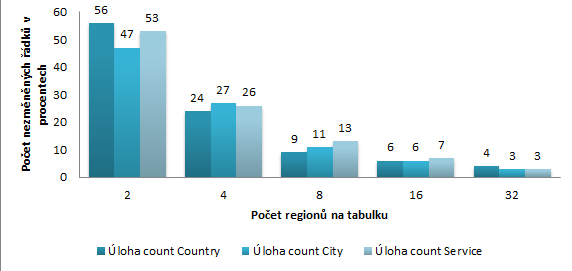
\includegraphics[width=1\textwidth, angle=0]{files/graf-presuny}
	\caption[Počet nepřesunutých řádků v závislosti na počtu regionů a MapReduce úloze]
	{Počet nepřesunutých řádků v závislosti na počtu regionů a MapReduce úloze}\label{fig:eko}
\end{figure}

\subsubsection{Výsledky měření počtu přesouvaných řádků při repartitioningu}
Pro každou konfiguraci jsem provedl měření třikrát, pokaždé na nově vygenerovaných datech a do tabulky jsem sepsal průměry těchto hodnot. K měření jsem používal datasety obsahující jeden milion řádků. Z měření jasně vyplývá, že u všech úloh došlo prakticky ke stejným přesunům, během vytváření nové tabulky. 

U úlohy na spočítání obyvatel v jednotlivých městech sice byli výsledky více rozkolísané než u zbylých dvou úloh, ale v průměru se ustálily na podobných hodnotách. To bylo zapříčiněno nejspíše tím, že řádky sice byly vzheldem ke struktuře dat již částečně seřazeny, dělící algoritmus však ne vždy rozdělil graf tak, aby tyto seřazené úseky zůstali na svém místě. Zde se nabízí budoucí úprava algoritmu tak, aby respektoval již částečnou data-locality. Tento přístup by pak mohl být aplikován především na provádění optimalizace na již v minulosti optimalizovaných tabulkách. V kombinaci s přístupem, kdy by se jen upravovala stávající tabulka namísto vytváření zcela nové by zde mohlo dojít k výraznému zrychlení při vytváření zoptimalizované tabulky.

Pro stávající řešení kdy se tabulka vytváři zcela znovu, není počet přesunutých řádků nijak podstatný. Jen se potvrdila domněnka z návrhu, že při rozřazování, dochází ke kompletnímu promíchání dat, a počet přesunutých řádků napříč regiony se odvíjí od počtu regionů, na kterých tabulka leží. Množství nepřesunutých dat totiž vždy odpovídá poměru dat k počtu regionů.
 
\subsection{Rozdíly v počtu emitovaných hodnot z mapperu}
Při druhém měření se zaměříme na rozdíly v počtech emitovaných výstupů z mapovací fáze. Pro zjištění rozdílů mezi počty emitovaných klíčů je zapotřebí přistoupit k měření jiným způsobem než je spuštění běžných mapreduce úloh. Protože v běžné úloze MapReduce se jako výstup z mapovací funkce emitují vždy všechny hodnoty nehledě na to, zda jsou stejné. Proto při vytváření úloh pro toto měření použijeme návrhový vzor "in-mapper combining", který provádí kombinační část už v rámci mapperu. Tím se zajistí, že z mapovací části vycházejí vždy již nasčítané unikátní klíče a lze provést vyhodnocení efektivity při optimalizaci.

\subsubsection{In-mapper combining}
Základní technika pro místní agregaci dat je combiner. Combiner poskytuje obecný mechanizmus, který slouží k redukování key-value párů vygenerovaných mapovací funkcí. Jedná se tedy víceméně o reducer, které zpracuje výsledek z jednoho mapperu. Při následná shuffle fázi pak dochází díky tomu k menšímu pohybu klíčů.\cite{inmemory}  Pseudokód takového postupu je uveden na obrázku \ref{fig:inmap}.

\begin{figure}[h]\centering
	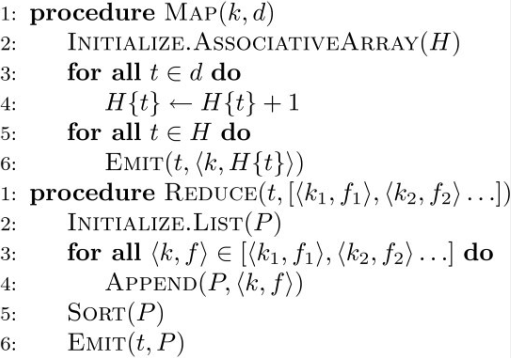
\includegraphics[width=0.6\textwidth, angle=0]{files/inmap}
	\caption[Pseudokód in-mapper combineru]
	{Pseudokód in-mapper combineru}\label{fig:inmap}
\end{figure}
Tento postup však neovlivňuje počet emitovaných  key-value párů z mapperu. Navíc  implementace Hadoopu nedává žádnou garanci kolikrát se daný combiner provede, a jestli vůbec k použítí reduceru dojde. 

Z toho důvodu se použije pro tuto úlohu In-mapper combining. Ten implementuje funkci combineru už v mapperu. Během zpracovávání dat dochází k postupnému ukládání key-value párů do mapy, kde se tyto hodnoty nasčítávají. Po zpracování se pak emitují jako výsledek mapovací funkce již zagregované data.

Tento návrhový vzor má v praktickém využití jedno velké omezení a to velikou paměťovou náročnost, kdy je potřeba v každém mapperu uchovávat mapu s postupně přibývajícími zagregovanými daty. Tento problém lze vyřešit periodickým emitováním části výsledků, vždy po zpracování $k$ výsledků. 

Vzhledem k tomu, že se v tomto případě nebudou zpracovávat úlohy, jež by zpracovávaly data s velkým množstvím unikátních klíčů, tak aplikování tohoto postupu není zapotřebí. Navíc by tento postup i zkreslil výsledky optimalizace. Proto použijeme variantu, kdy se z každého mapperu emitují již kompletně zagregované výsledky.

\subsubsection{Konfigurace testovacích dat}
Při tomto měření využijeme data vygenerovaná při předchozím měření. Pro každou z pěti konfigurací nejdříve provedeme tři testovací úlohy. Pro tyto úlohy zaznamenáme počet emitovaných hodnot z mapperu, který je uveden ve statistikách o běhu úlohy. V defaultním nastavení HBase se vytvoří pro každý region v tabulce nový mapper. Počet mapperu tedy kopíruje počet regionů na kterých tabulka leží. Tím zaznamenáme počty emitovaných klíčů pro všechny úlohy a tabulky. Během provádění úloh, jsme zároveň ukládali i metadata potřebná k repartitioningu.

Po zaznamenání všech výsledků je na řadě vytvořit z nashromážděných metadat nové zoptimalizované tabulky. Nakonec se celý proces měření opakuje i na těchto tabulkách. Můžeme tedy přistoupit k porovnání zjištěných výsledků a k jejich vyhodnocení.

\paragraph{Výsledky měření rozdílů v počtech emitovaných klíčů}
Výsledky měření potvrdili, že optimalizace má pozitivní efekt na data-locality v rámci Regionů. V kombinaci s využitím in-mapper combineru, lze dosáhnout výrazného úbytku přenášených dat při shuffling fázi oproti neoptimalizovaným datům. Z měření však vyplynulo, že dosažená efektivita velmi souvisí jak se strikturou zpracovávaných dat, tak na typu dotazů, které se nad daty provádějí.

Při první úloze došlo k výraznému úbytku emitovaných klíčů, jak je vidět na grafu\ref{fig:mesta}. Se zvyšujícím se počtem regionů a tedy mapovacích funkcí, se postupně zvyšovala i data-locality. Což se projevilo větším poměrem v rozdílech mezi výsledky u optimalizovaných a neoptimalizovaných dat

\begin{figure}[h]\centering
	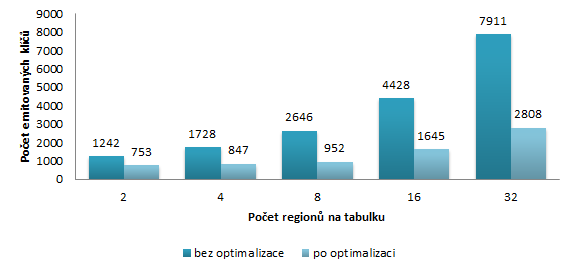
\includegraphics[width=1\textwidth, angle=0]{files/mesta}
	\caption[Výsledky úlohy pro spočítání měst]
	{Výsledky úlohy pro spočítání měst}\label{fig:mesta}
\end{figure}

V úloze pro spočtení krajů došlo k ještě většímu úbytku emitovaných klíčů. To je ale zapříčiněno především malým počtem výsledné zagregované množiny dat. V tomto případě například při konfiguraci o 32 regionech, tedy o 32 mapperech, vycházejí na každou výslednou hodnotu v průměru 2 mappery. Díky tomu dochází prakticky k emitování 1 až 2 zagregovaných klíčů z mapperu. Nutno dodat, že tato úloha je vyřešená s výbornými výsledky i za použití pouze in-mapper combineru. Ušetřené kapacity jsou i přes to, že samotné srovnání vypadá velmi efektivně, zanedbatelné. Výsledky jsou uvedeny na grafu\ref{fig:kraje}. 
\begin{figure}[h]\centering
	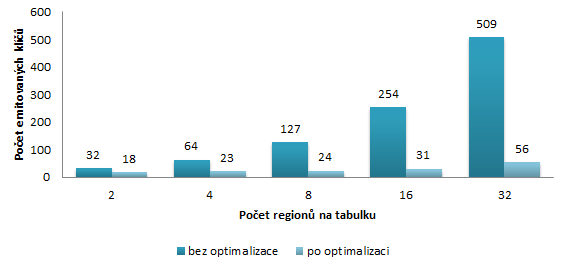
\includegraphics[width=1\textwidth, angle=0]{files/kraje}
	\caption[Výsledky úlohy pro spočítání krajů]
	{Výsledky úlohy pro spočítání měst}\label{fig:kraje}
\end{figure}
Poslední měřená úloha nevykázala téměř žádný rozdíl v emitovaných klíčích jak je vidět v grafu \ref{fig:sluzby}. Je to zapříčiněno především malý počtem výsledků úlohy a také tím, že jednotlivé řádky emitují více rozdílných klíčů a tím se na reparitioning kladou protichůdné požadavky. Emitování více klíčů samo o sobě není problémem, problém je především struktura dat, kdy jednotlivé klíče jsou zastoupeny v datech rovnoměrně. Při takto malém počtu to prakticky nedovoluje vytvoření větších seskupení řádku, které emitují jen jeden či jen několik klíčů. Tento příklad také simuluje situaci po provedení otimalizace na základě dat z více rozdílných úloh, které se vyznačují při optimalizaci protichůdnými požadavky na strukturu dat.
\begin{figure}[h]\centering
	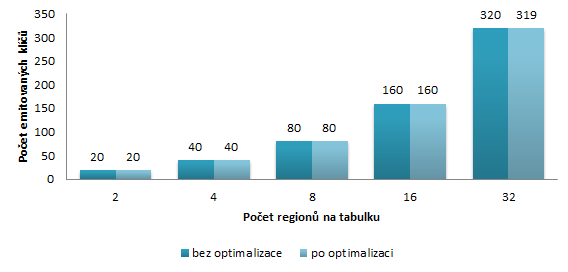
\includegraphics[width=1\textwidth, angle=0]{files/sluzby}
	\caption[Výsledky úlohy pro spočítání služeb]
	{Výsledky úlohy pro spočítání služeb}\label{fig:sluzby}
\end{figure}

\subsection{Shrnutí}
Z provedených měření vyplývá, že repatitioning vede k jistému snížení přenosu dat. Nicméně tyto výsledky jsou velmi závislé na struktuře dat a také na úlohách pro které jsou optimalizované. Na základě toho lze říci, že toto řešení není cesta, která by obecně vedla k úspoře datových přenosů při vykonávání mapreduce úloh. Na specifické úlohy se však může aplikovat s uspokojivými výsledky. Především v situacích, kde je možné k zpracování dat použít úlohy vytvořené na bázi in-mapper controleru je i v nynějším stavu řešení možné dosáhnout výrazného ubýtku přenášených dat.

Je třeba také uvést, že bez vyřešení problému fyzického ukládání dat pro regiony a tím i bez možnosti efektivně rozvrhovat redukční úlohy,  nelze plně těžit ze všech výhod, které by jsme jinak díky repartitioningu získali.




\section{Testování}
V této kapitole budou popsány metody, kterými jsem otestoval naimplementované řešení a mapreduce úlohy, které jsem využíval k vyhodnocení výsledků práce. Poté budou poskytnuty výsledky těchto testů.
K otestování jsem využil tyto postupy:
\begin{itemize}
	\item Manuální testy
	\item JUnit testy
	\item MRUnit testy
\end{itemize}

\subsection{Manuální testy}
\subsection{JUnit testy}
\subsection{MRUnit testy}
Testování za pomocí MRUnit testů je založeno na JUnit testování a využívá se k testování Map Reduce programů od verze 0.20 \cite{mrunit}... 
\subsection{Výsledky testů}
    % jednoduchá tabulka
    \begin{tabbing}
    Testovaná část ~~~~\= počet testů ~~~~
     \kill
    \bfseries Testovaná část \>
    \bfseries Počet testů  
     \\[2mm]
    monitoring \> xx\\
    repartitioning\> xx \\
    Map-Reduce joby \> xx
    \end{tabbing}

\begin{conclusion}
	%sem napište závěr Vaší práce
\end{conclusion}

\bibliographystyle{csn690}
\bibliography{mybibliographyfile}

\appendix

\chapter{Generátor zkušebních dat}\label{ch:generator}
Pro potřeby testování bylo nezbytné obstarat vhodná dat na kterých by se mohla implementace vyzkoušet. Nakonec jsem se rozhodl použít kompletně vygenerovaná data a to především kvůli nutnosti mít datasety o specifických vlastnostech. Proto jsem napsal generátor dat, který generuje data odpovídající smyšlenému seznamu osob v ČR. U těchto osob je jako klíč bráno unikátní rodné číslo. Každá osoba má určenou obec okres a kraj, určené podle reálných dat o počtech obyvatel v těchto celcích. Všechny tyto údaje jsou uloženy ve family \texttt{osoba}. Druhá family \texttt{sluzba} obsahuje defaultně 10 sloupců pojmenovaných \texttt{rok2000} až \texttt{rok2009}. Tyto sloupce obsahují náhodné hodnoty v rozmezí \texttt{sluzba\_cislo\_1} až \texttt{sluzba\_cislo\_9}. U každého sloupce je možné nastavit hustotu zaplnění sloupce. Výsledná řádek tedy může mít následující strukturu \ref{fig:hue}.
\begin{figure}[h]\centering
	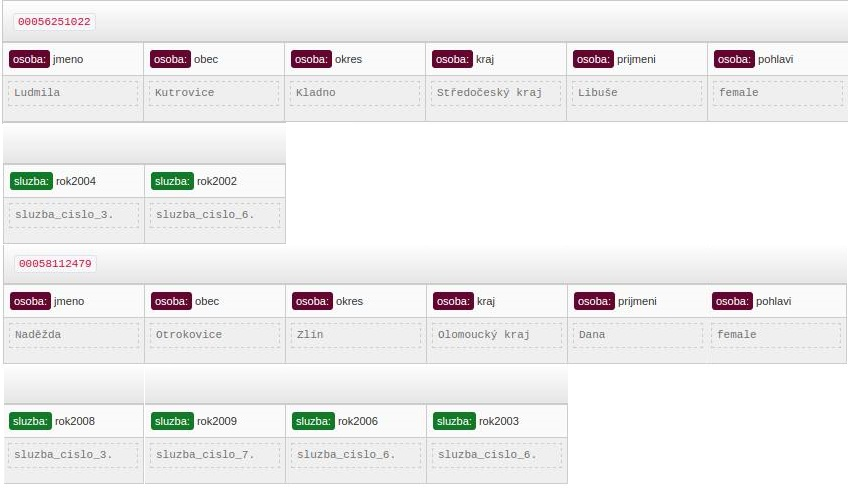
\includegraphics[width=1\textwidth, angle=0]{files/hue}
	\caption[Dva vygenerované řádky pomocí generátoru dat]
	{Dva vygenerované řádky pomocí generátoru dat}\label{fig:hue}
\end{figure} 

Dále je zde možnost navolit si počet regionů v nové databázi, což je při testování přesunů dat mezi regiony žádoucí. Pro zjišťení, k jakému pohybu řádků mezi regiony dochází při repartitioningu lze přidat před rodné číslo v identifikátoru řádku i prefix značící region, na kterém je umístěn. 

Parametry nově vzniklé databáze se nastavují v kódu, vzhledem k tomu, že při generování dat bude požadovaná další konkrétní úprava, například přidání specifických sloupců atd. V následujícím bloku je ukázka nastavení proměnných pro vygenerování datasetu o 100 000 řádcích. \pagebreak

\begin{lstlisting}[frame=single]  % Start your code-block

String databaseName = "test-100k-pretfix";
int setMaxPopulationInCity = 100000;
int setMaxGeneratedRows = 1000000;
int numOfServices =10; 
boolean manageRegions = true;
boolean hasPrefix = true;
        
int numOfRegions = 5;  //pocet regionu pouzije se i u urcovani prefixu
int[] serviceDensity = new int[10];
serviceDensity[0] = 10;  //nastaveni hustoty zalneni u sloupce rok2000
serviceDensity[1] = 10;  //nastaveni hustoty zalneni u sloupce rok2001
serviceDensity[2] = 50;  //nastaveni hustoty zalneni u sloupce rok2002
serviceDensity[3] = 50;  //nastaveni hustoty zalneni u sloupce rok2003
serviceDensity[4] = 50;  //nastaveni hustoty zalneni u sloupce rok2004
serviceDensity[5] = 50;  //nastaveni hustoty zalneni u sloupce rok2005
serviceDensity[6] = 0;   //nastaveni hustoty zalneni u sloupce rok2006
serviceDensity[7] = 0;   //nastaveni hustoty zalneni u sloupce rok2007
serviceDensity[8] = 100; //nastaveni hustoty zalneni u sloupce rok2008
serviceDensity[9] = 100; //nastaveni hustoty zalneni u sloupce rok2009
\end{lstlisting}        


\chapter{Instalace Hadoop prostředí}
I přes to, že lze dohledat několik návodů jak postupovat při instalaci Hadoopu, konkrétně jeho distribuce Cloudera 5.3.0. Myslím, že i přes to je na místě zde uvést takový návod. Pomocí tohoto návodu je možné nainstalovat Hadoop v pseudodistribuovaném módu na systém Ubuntu 14.04. Je uveden postup pro instalaci na čistou instalaci Ubuntu, není tedy potřeba nastavovat nic dalšího. Při instalaci jsem postupoval především podle návodu na  \texttt{https://bitbucket.org/barseghyanartur/simple-cloudera-install} a doplnil jsem ho o několik informací.

\section{Příprava na instalaci}
Ještě před samotnou instalací je zapotřebí nejdříve nainstalovat potřebné programy a nastavit systém.
Jako první nainstalujeme ssh.
\begin{lstlisting}[frame=single]  % Start your code-block

    $ sudo apt-get install ssh
    $ sudo apt-get install rsync
    $ sudo apt-get install openssh-server
    $ ssh-keygen -t dsa -P '' -f ~/.ssh/id_dsa
    $ cat ~/.ssh/id_dsa.pub >> ~/.ssh/authorized_keys
    $ sudo chmod 600 ~/.ssh/id_dsa
    $ sudo chmod 600 ~/.ssh/id_dsa.pub
    $ sudo service ssh start
\end{lstlisting} 
Přidáme nového uživatele a nastavíme mu heslo:
\begin{lstlisting}[frame=single]  % Start your code-block

$ sudo useradd cloudera
$ sudo passwd cloudera
\end{lstlisting} 

\pagebreak
Poté stáhneme soubory, sloužící k vytvoření a nastavení složek pro instalaci. Tyto skripty jsou dostupné na následující adrese:
\begin{lstlisting}[frame=single]  % Start your code-block

http://bitbucket.org/barseghyanartur/ simple-cloudera-install/get/tip.tar.gz
\end{lstlisting} 

Tyto skripty rozbalíme a spustíme, tím se vytvoří potřebná struktura adresářů pro instalaci
\begin{lstlisting}[frame=single]  % Start your code-block

$ tar -xvzf tip.tar.gz
$ chmod +x scripts/create_dirs.sh
$ sudo ./scripts/create_dirs.sh cloudera
\end{lstlisting} 

Přidáme nově vytvořeného uživatele do skupiny:
\begin{lstlisting}[frame=single]  % Start your code-block

$ sudo adduser cloudera sudo
\end{lstlisting}

Cloudera vyžaduje k instalaci uživatele, který má administrátorská práva a zároveň nemá nastavené heslo. Proto musíme dočasně změnit chování sudoers skupiny. Po nainstalování Cloudery je pak z bezpečnostních důvodů nezbytné tuto změnu vrátit zpět. Otevřeme tedy soubor:

\begin{lstlisting}[frame=single]  % Start your code-block

$ sudo nano /etc/sudoers
\end{lstlisting}
a nahradíme tento řádek:
\begin{lstlisting}[frame=single]  % Start your code-block

%sudo ALL=(ALL:ALL)
\end{lstlisting}
následujícím řádkem:
\begin{lstlisting}[frame=single]  % Start your code-block

%sudo ALL=(ALL:ALL) NOPASSWD: ALL
\end{lstlisting}

Dále přepneme na nového uživatele \texttt{cloudera} a  vygenerujeme pro něj SSH klíč:
\begin{lstlisting}[frame=single]  % Start your code-block

$ sudo su cloudera
$ ssh-keygen -t dsa -P '' -f ~/.ssh/id_dsa
$ cat ~/.ssh/id_dsa.pub >> ~/.ssh/authorized_keys
$ cat ~/.ssh/id_dsa.pub|xclip -i
$ sudo chmod 600 ~/.ssh/id_dsa
$ sudo chmod 600 ~/.ssh/id_dsa.pub
$ sudo service ssh restart
\end{lstlisting}

Nastavíme specifikované doménové jméno počítače například následovně:
\begin{lstlisting}[frame=single]  % Start your code-block

$ sudo nano /etc/hosts
> 217.21.196.178 hadoop.example.com hdp
$ sudo nano /etc/hostname/
> hdp
\end{lstlisting}

Nainstalujeme Python Avro
\begin{lstlisting}[frame=single]  % Start your code-block

$ sudo apt-get install python-virtualenv
$ sudo apt-get install python-setuptools
$ sudo easy_install virtualenv
$ sudo easy_install avro
\end{lstlisting}
Ujistíme se, že máme vypnutý firewall:
\begin{lstlisting}[frame=single]  % Start your code-block

$ sudo service firewall stop
\end{lstlisting}
Ověříme, že námi definovaný hostname je dostupný:
\begin{lstlisting}[frame=single]  % Start your code-block

$ python -c 'import socket; print socket.getfqdn(), socket.gethostbyname(socket.getfqdn())'
\end{lstlisting}
Odpověď by měla obsahovat námi definované jméno.
Nakonec spustíme automatický installer:
\begin{lstlisting}[frame=single]  % Start your code-block

$ cd distrib/cloudera/
$ chmod +x cloudera-manager-installer.bin
$ sudo ./cloudera-manager-installer.bin
\end{lstlisting}

Ještě před pokračováním v instalaci provedeme následující příkazy:
\begin{lstlisting}[frame=single]  % Start your code-block

$ virtualenv /usr/lib/cmf/agent/build/env
$ sudo su cloudera
$ ssh hadoop.example.com
$ ssh hdp
\end{lstlisting}

Nyní už můžeme pokračovat podle pokynu na webové instalaci na adrese:
\begin{lstlisting}[frame=single]  % Start your code-block

localhost:7180/cmf/home
\end{lstlisting}

Po dokončení instalace, by již nemělo nic bránit k startu Hadoopu. Detailněji popsaná samotná instalace cloudery je popsaná přímo v manuálu na stránkách Cloudery:
\begin{lstlisting}[frame=single]  % Start your code-block

http://www.cloudera.com/content/cloudera/en/documentation/core/latest /topics/installation_installation.html
\end{lstlisting}
\chapter{Seznam použitých zkratek}
% \printglossaries
\begin{description}
	\item[HDFS] Hadoop Distributed File System
	\item[REST] Representational State Transfer
	\item[CRUD] Create Read Update Delete
	\item[API] Application Programming Interface
	\item[SQL] Structured Query Language
	\item[NoSQL] Not only SQL
	\item[DBMS] DataBase Management System
	\item[RDBMS] Relational DataBase Management System
	\item[WAL] Write-Ahead Log
	

\end{description}


\chapter{Obsah přiloženého CD}

%upravte podle skutecnosti

\begin{figure}
	\dirtree{%
		.1 readme.txt\DTcomment{stručný popis obsahu CD}.
		.1 exe\DTcomment{adresář se spustitelnou formou implementace}.
		.1 src.
		.2 impl\DTcomment{zdrojové kódy implementace}.
		.2 thesis\DTcomment{zdrojová forma práce ve formátu \LaTeX{}}.
		.1 text\DTcomment{text práce}.
		.2 thesis.pdf\DTcomment{text práce ve formátu PDF}.
		.2 thesis.ps\DTcomment{text práce ve formátu PS}.
	}
\end{figure}

\end{document}
